Este manual tiene como objetivo proporcionarte una guía detallada sobre cómo utilizar todas las características y funcionalidades de nuestra aplicación.
Nuestra aplicación está diseñada para ser accesible a través de la web y desde la app móvil, por lo que habrá algunas diferencias en la interfaz y en la forma de interactuar con la aplicación dependiendo del dispositivo que utilices.

\subsubsection{Requisitos del Sistema}
Antes de comenzar, asegúrate de que tu dispositivo cumple con los siguientes requisitos:

\begin{itemize}
	\item Navegador web móvil actualizado (recomendamos Google Chrome o Mozilla Firefox) o la app instalada.
	\item Conexión a Internet estable.
	\item Resolución de pantalla mínima de 375x667 píxeles.
\end{itemize}

\subsubsection{Acceso a la Página Web}
En caso de no tener app instalada, acceder a nuestra página web siguiendo estos pasos:

\begin{enumerate}
	\item Abre tu navegador web.
	\item En la barra de direcciones, ingresa la URL de nuestro sitio web: www.astour.online.
	\item Presiona Enter.
\end{enumerate}

\subsubsection{Funcionalidades Principales}
A continuación, describiremos las funcionalidades principales:

\subsubsection{Autenticación}
\hrulefill
\subsubsection{Registro de Usuario}
Si eres un guía o un nuevo administrador pide a un administrador que te cree una cuenta.
De lo contrario, registrarte siguiendo estos pasos:

\begin{enumerate}
	\item Accede al apartado de cuenta. Mirar figuras \ref{fig:cuenta-movil}, \ref{fig:cuenta-app}, \ref{fig:cuenta-web}.
	\item Se abrirá un modal con un formulario para iniciar sesión y un enlace en la parte inferior para registrarte como nuevo usuario.
	      Haz clic sobre el enlace “Registrate aquí” para acceder al formulario de registro. Mirar figura \ref{fig:inicio-form}.
	\item Completa el formulario de registro con tu información personal y pulsa el botón “Registrarse” para enviar el formulario. Mirar figura \ref{fig:registro-form}.
\end{enumerate}

Al completar el registro con éxito, accederás automáticamente a tu cuenta.


\subsubsection{Inicio de Sesión}
Si ya tienes una cuenta, puedes iniciar sesión siguiendo estos pasos:

\begin{enumerate}
	\item Accede al apartado de cuenta. Mirar figuras \ref{fig:cuenta-movil}, \ref{fig:cuenta-app}, \ref{fig:cuenta-web}.
	\item Se abrirá un modal con un formulario para iniciar sesión.
	      Ingresa tu email y contraseña en los campos correspondientes y pulsa el botón “Iniciar Sesión” para acceder a tu cuenta. Mirar figura \ref{fig:inicio-form}.
\end{enumerate}

\begin{figure}[H]
	\centering
	\begin{minipage}{0.45\textwidth}
		\centering
		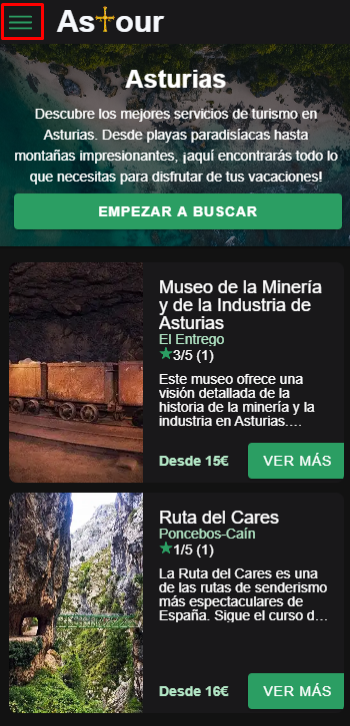
\includegraphics[width=0.45\textwidth]{7-Construccion/Manuales/mobile/menu marcado.png}
		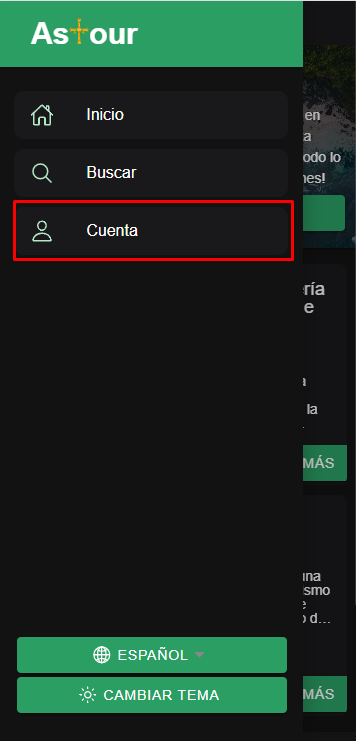
\includegraphics[width=0.45\textwidth]{7-Construccion/Manuales/mobile/cuenta marcado.png}
		\caption{Autenticación \\ Despliegue del menú y selección de la opción “Cuenta” .}
		\label{fig:cuenta-movil}
	\end{minipage}
	\hfill
	\begin{minipage}{0.45\textwidth}
		\centering
		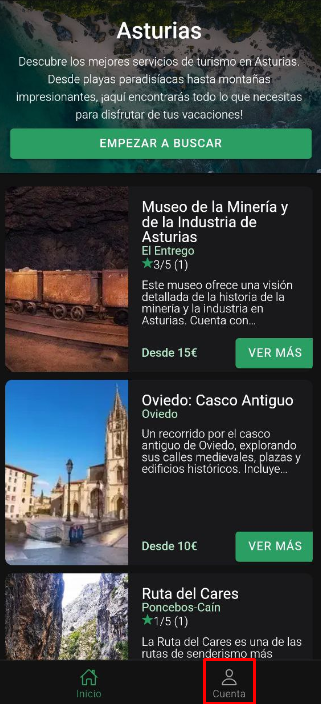
\includegraphics[width=0.45\textwidth]{7-Construccion/Manuales/app/P1-Registro.png}
		\caption{Autenticación \\ Selección de la opción “Cuenta” de la barra inferior de navegación.}
		\label{fig:cuenta-app}
	\end{minipage}
\end{figure}
\begin{figure}[H]
	\centering
	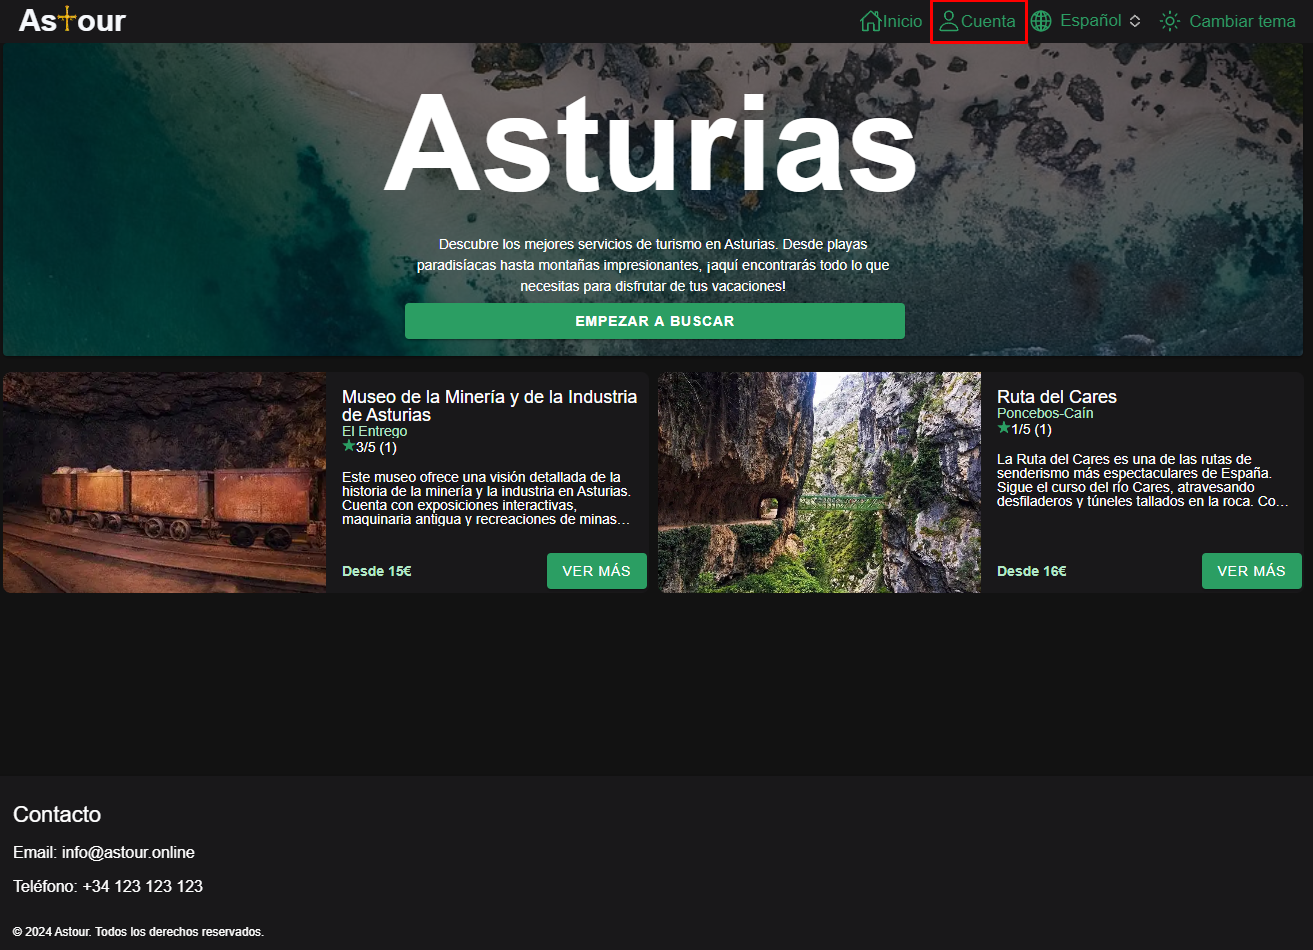
\includegraphics[width=0.5\textwidth]{7-Construccion/Manuales/web/cuenta opcion.png}
	\caption{Autenticación \\ Selección de la opción “Registrarse” .}
	\label{fig:cuenta-web}
\end{figure}

\begin{figure}[H]
	\centering
	\begin{minipage}{0.45\textwidth}
		\centering
		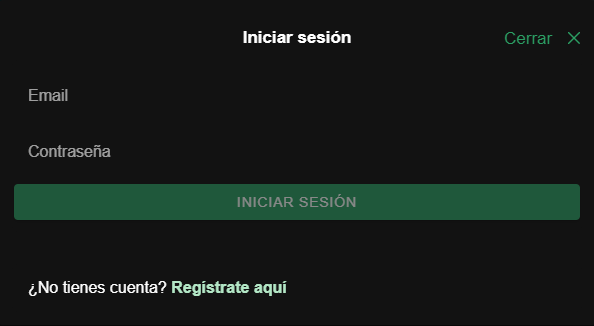
\includegraphics[width=1\textwidth]{7-Construccion/Manuales/web/modal inicio.png}
		\caption{Autenticación \\ Modal de inicio de sesión.}
		\label{fig:inicio-form}
	\end{minipage}
	\hfill
	\begin{minipage}{0.45\textwidth}
		\centering
		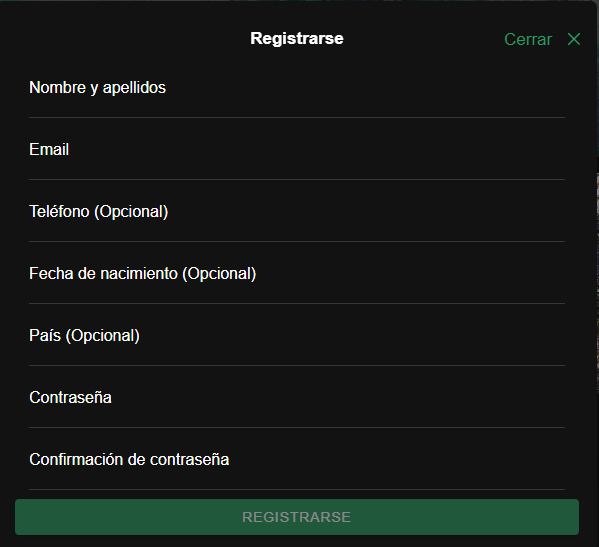
\includegraphics[width=1\textwidth]{7-Construccion/Manuales/web/modal registro.png}
		\caption{Autenticación \\ Modal de registro de sesión.}
		\label{fig:registro-form}
	\end{minipage}
\end{figure}


\subsubsection{Exploración de Actividades}
\hrulefill
\subsubsection{Buscar Actividades}

Desde la página de inicio, puedes buscar las actividades pulsando el botón “Empezar a buscar” . Mirar figura \ref{fig:inicio-buscar}.
\\ \\[1ex]
Te llevará a una página donde encontrarás una lista de actividades disponibles, con la opción de filtrar por nombre, por rango de fechas, precio máximo, número de personas, puntuación mínima y idioma.
Mirar figura \ref{fig:buscar-actividades}.
\\ \\[1ex]
Para filtrar por nombre, ingresa el nombre de la actividad en la barra de búsqueda superior. A los 3 segundos de haber dejado de escribir, se mostrarán las actividades que coincidan con el nombre ingresado. Mirar \ref{fig:buscar-nombre}.
\\ \\[1ex]
Para filtrar por una características más específicas, haz uso del meú de filtros. Mirar figura \ref{fig:filtros-menu}.
\\ \\[1ex]
En caso de estar desde dispositivo móvil, para llegar a ese menú se deberá pulsar el botón “Añadir filtros” que se encuentra en la parte inferior de la pantalla. Mirar figura \ref{fig:filtros-movil}.
\\ \\[1ex]
Para filtrar por rango de fechas, selecciona las fechas de inicio y fin en los campos correspondientes.
Para filtrar por precio máximo, ajusta el control deslizante.
Para filtrar por número de personas, utiliza los botones de incremento y decremento.
Para filtrar por puntuación mínima, utiliza los botones de incremento y decremento.
Para filtrar por idioma, selecciona los idiomas deseados tocando las casillas correspondientes.
\\ \\[1ex]
Para aplicar los filtros específicos, pulsa el botón “Añadir filtros” que se encuentra en la parte inferior del menú de filtros. Mirar figura \ref{fig:añadir-filtros}.
En el caso que desees modificar los filtros aplicados, vuelve a pulsar el botón “Añadir filtros” después de haber seleccionado los filtros deseados.
\\ \\[1ex]
Una vez aplicados los filtros deseados, se mostrarán las actividades que coincidan con los filtros aplicados.
\\ \\[1ex]
En caso de que desees hacer modificaciones o borrar los filtros, deberás pulsar el botón “Eliminar filtros” . Mirar figura \ref{fig:eliminar-filtros}.

\begin{figure}[H]
	\centering
	\begin{minipage}{0.45\textwidth}
		\centering
		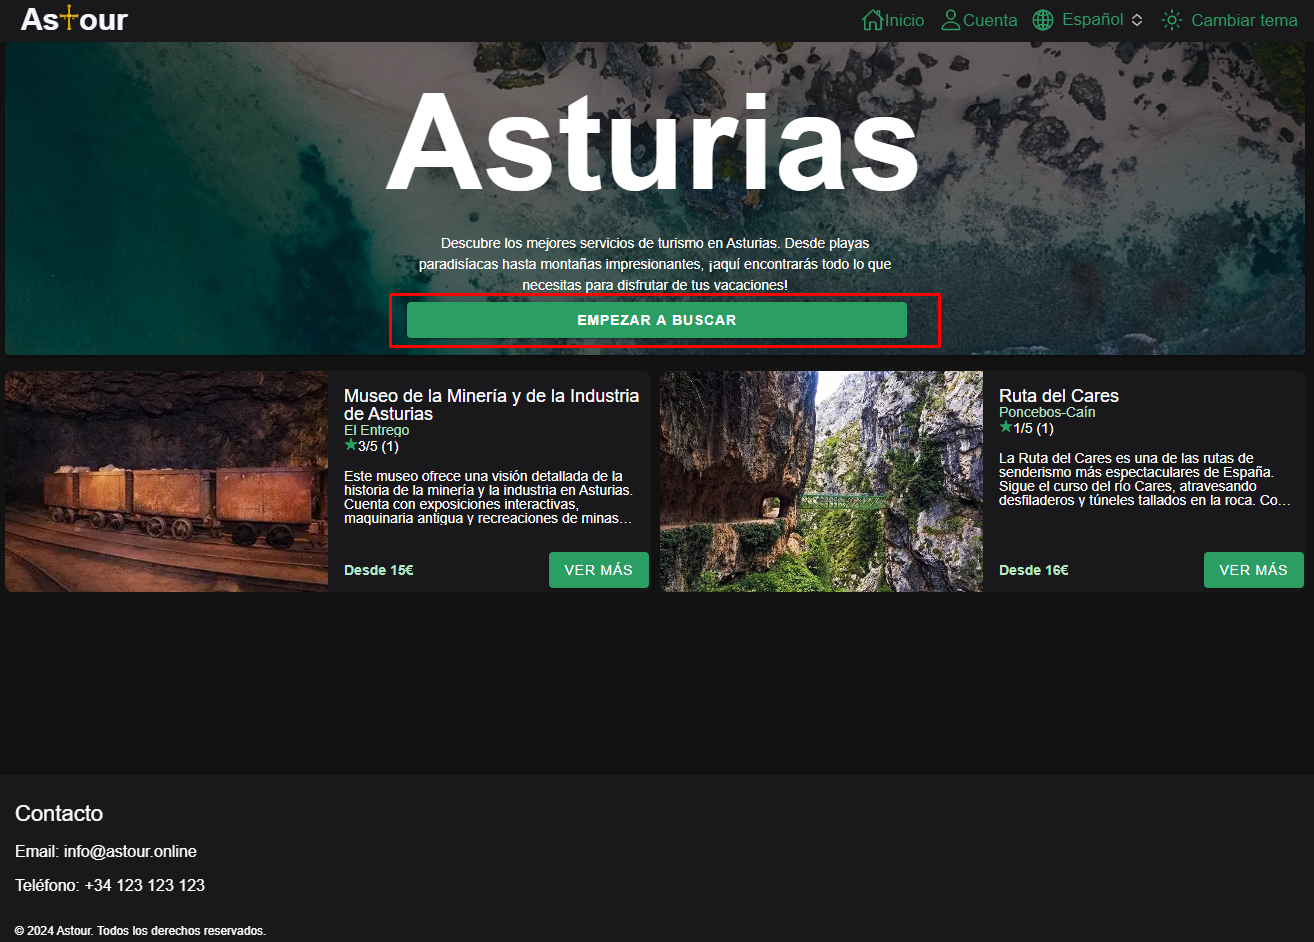
\includegraphics[width=1\textwidth]{7-Construccion/Manuales/web/inicio buscar.png}
		\caption{Exploración de Actividades \\ Botón para buscar actividades.}
		\label{fig:inicio-buscar}
	\end{minipage}
	\hfill
	\begin{minipage}{0.45\textwidth}
		\centering
		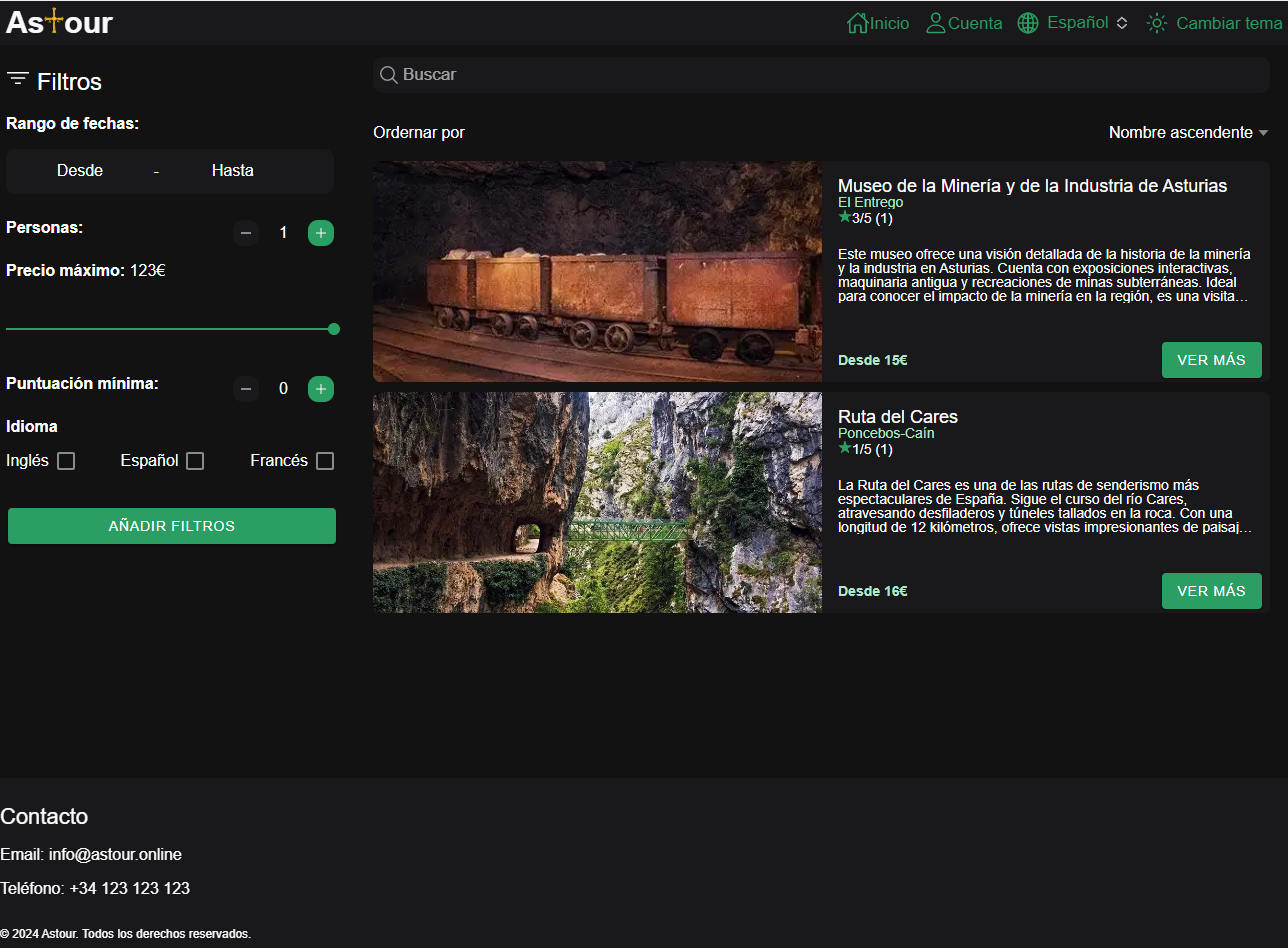
\includegraphics[width=1\textwidth]{7-Construccion/Manuales/web/buscar actividades.png}
		\caption{Exploración de Actividades \\ Listado de actividades}
		\label{fig:buscar-actividades}
	\end{minipage}
\end{figure}

\begin{figure}[H]
	\centering
	\begin{minipage}{0.45\textwidth}
		\centering
		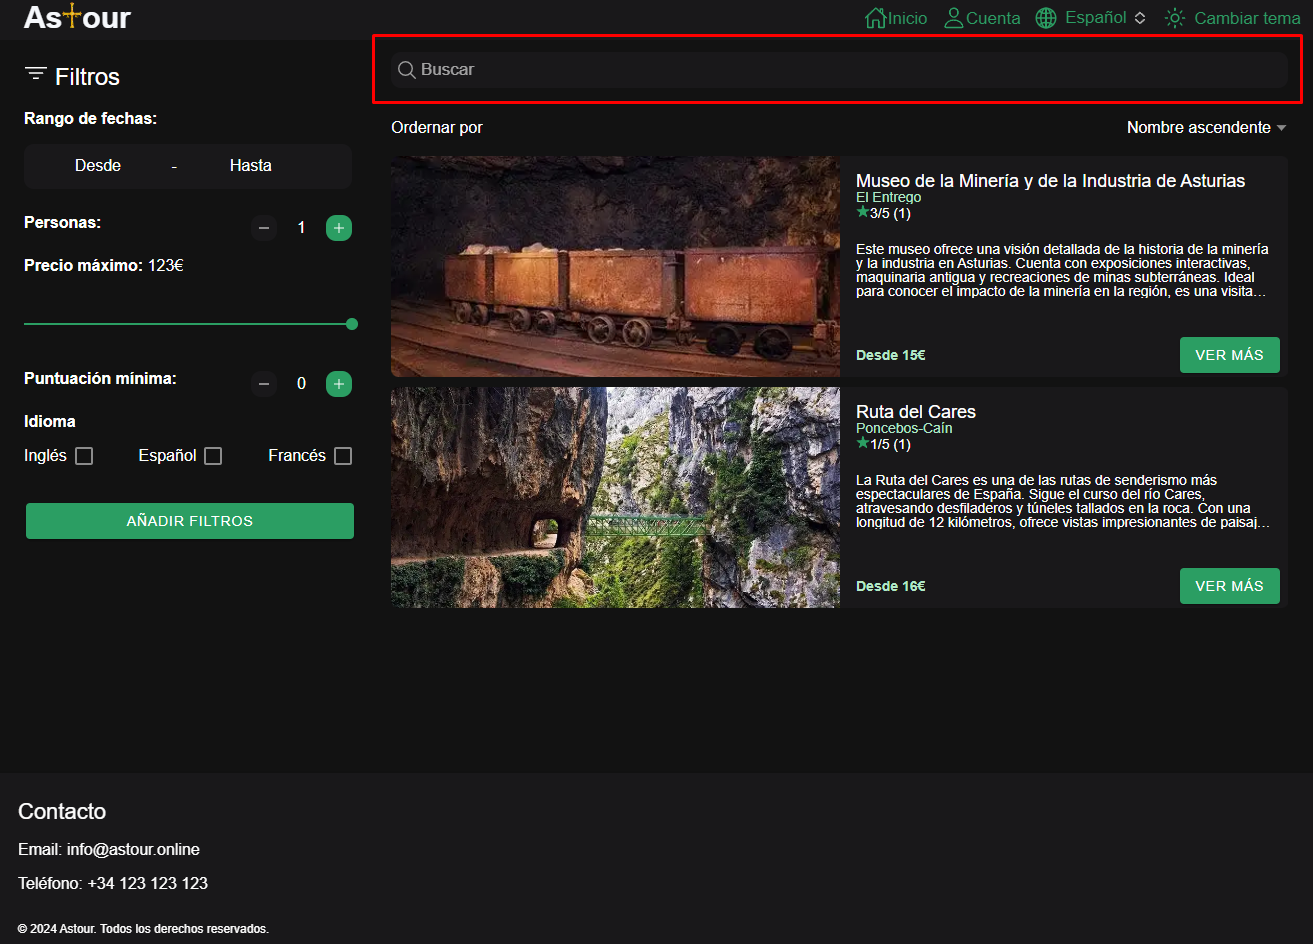
\includegraphics[width=1\textwidth]{7-Construccion/Manuales/web/buscar nombre.png}
		\caption{Exploración de Actividades \\ Buscar por nombre}
		\label{fig:buscar-nombre}
	\end{minipage}
	\hfill
	\begin{minipage}{0.45\textwidth}
		\centering
		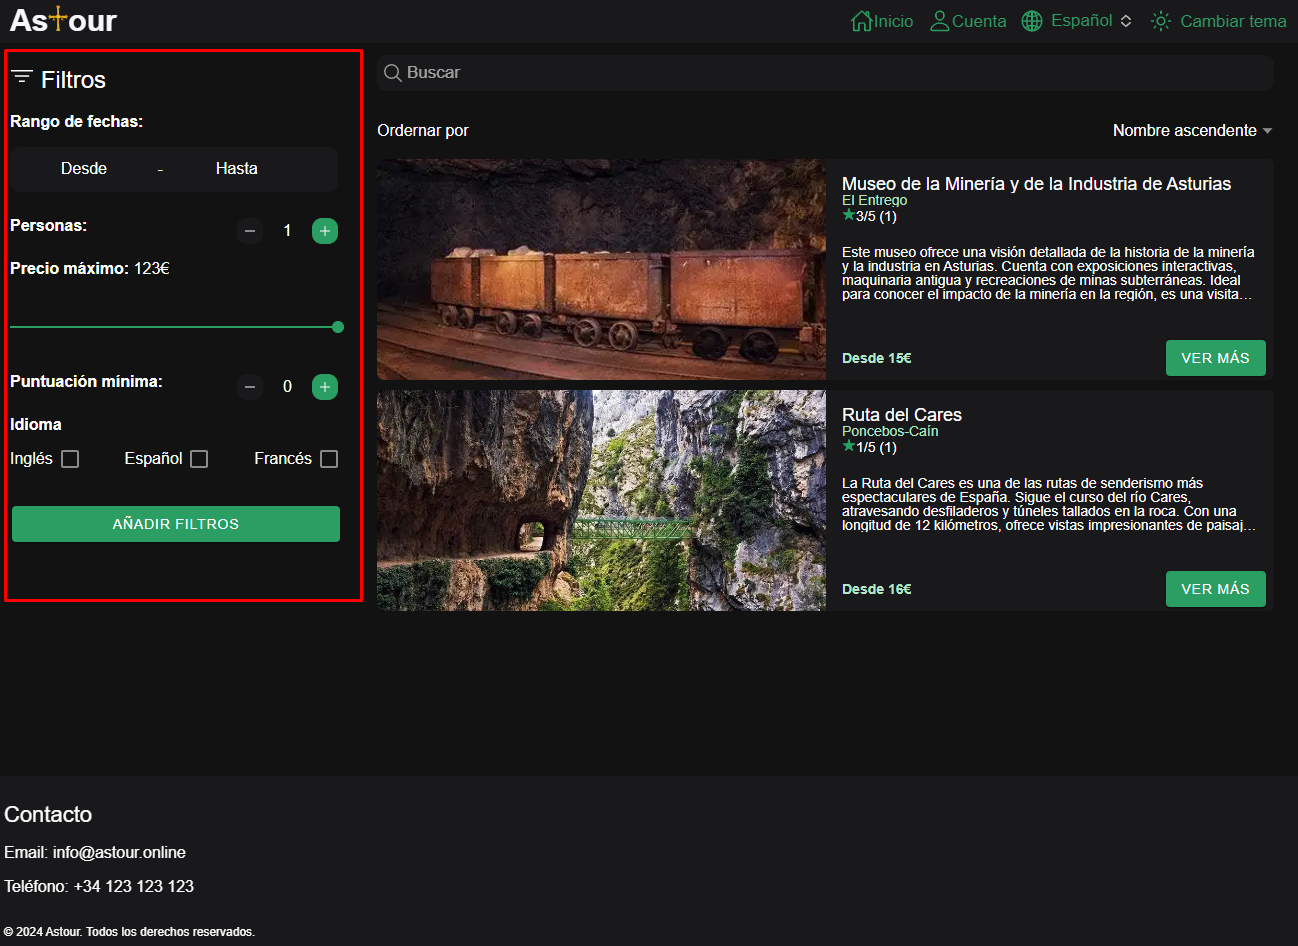
\includegraphics[width=1\textwidth]{7-Construccion/Manuales/web/menu filtros.png}
		\caption{Exploración de Actividades \\ Menú de filtros}
		\label{fig:filtros-menu}
	\end{minipage}
\end{figure}


\begin{figure}[H]
	\centering
	\begin{minipage}{0.45\textwidth}
		\centering
		\includegraphics[width=0.45\textwidth]{7-Construccion/Manuales/mobile/añadir filtros.png}
		\caption{Exploración de Actividades \\ Abrir menú de filtros}
		\label{fig:filtros-movil}
	\end{minipage}
	\hfill
	\begin{minipage}{0.45\textwidth}
		\centering
		\includegraphics[width=1\textwidth]{7-Construccion/Manuales/web/añadir filtros.png}
		\caption{Exploración de Actividades \\ Añadir filtros}
		\label{fig:añadir-filtros}
	\end{minipage}
\end{figure}

\begin{figure}[H]
	\centering
	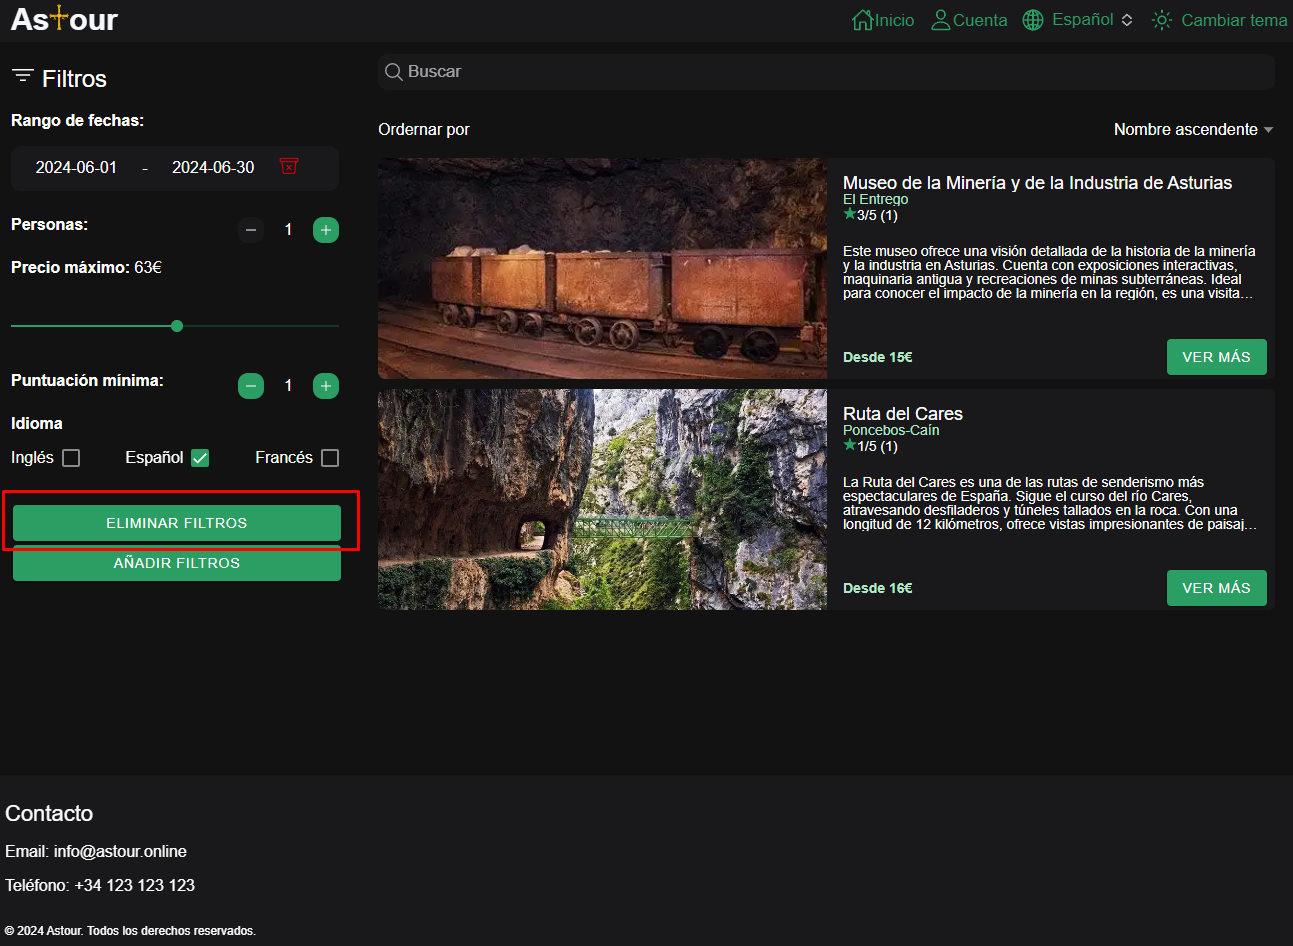
\includegraphics[width=0.5\textwidth]{7-Construccion/Manuales/web/eliminar filtros.png}
	\caption{Exploración de Actividades \\ Eliminar filtros}
	\label{fig:eliminar-filtros}
\end{figure}


\subsubsection{Ver Información Detallada de una Actividad}
Para ver la información detallada de una actividad, pulsa el botón “Ver más” de la actividad deseada.
Mirar figura \ref{fig:ver-info}.
\\ \\[1ex]
Se abrirá una nueva ventana con la información detallada de la actividad, incluyendo el nombre, la descripción, la duración, la puntuación y la ubicación.
Mirar figura \ref{fig:detalles-actividad}.
\\ \\[1ex]
Para ver los precios, idiomas y horarios de la actividad, pulsa el botón “Ver disponibilidad” que se encuentra bajo la descripción de la actividad.
Mirar figura \ref{fig:ver-disponibilidad}.
\\ \\[1ex]
Podrás seleccionar la fecha en el calendario y el número de personas usando los botones de incremento y decremento.
Una vez seleccionada la fecha y el número de personas, podrás ver los precios, idiomas y horarios disponibles para la actividad.
Mirar figura \ref{fig:disponibilidad}.


\begin{figure}[H]
	\centering
	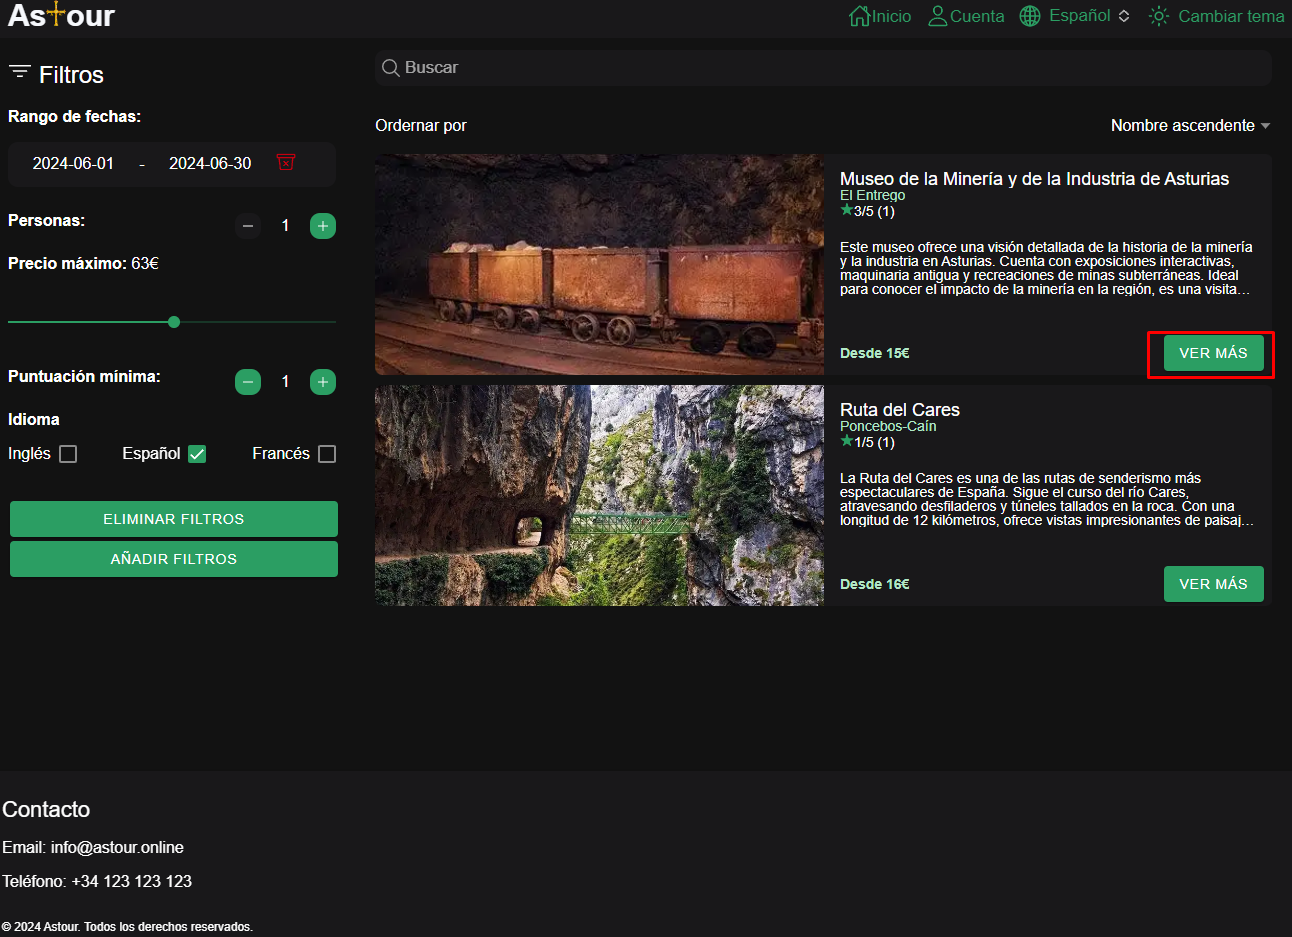
\includegraphics[width=0.5\textwidth]{7-Construccion/Manuales/web/ver info.png}
	\caption{Exploración de Actividades \\ Ver información detallada}
	\label{fig:ver-info}
\end{figure}

\begin{figure}[H]
	\centering
	\begin{minipage}{0.45\textwidth}
		\centering
		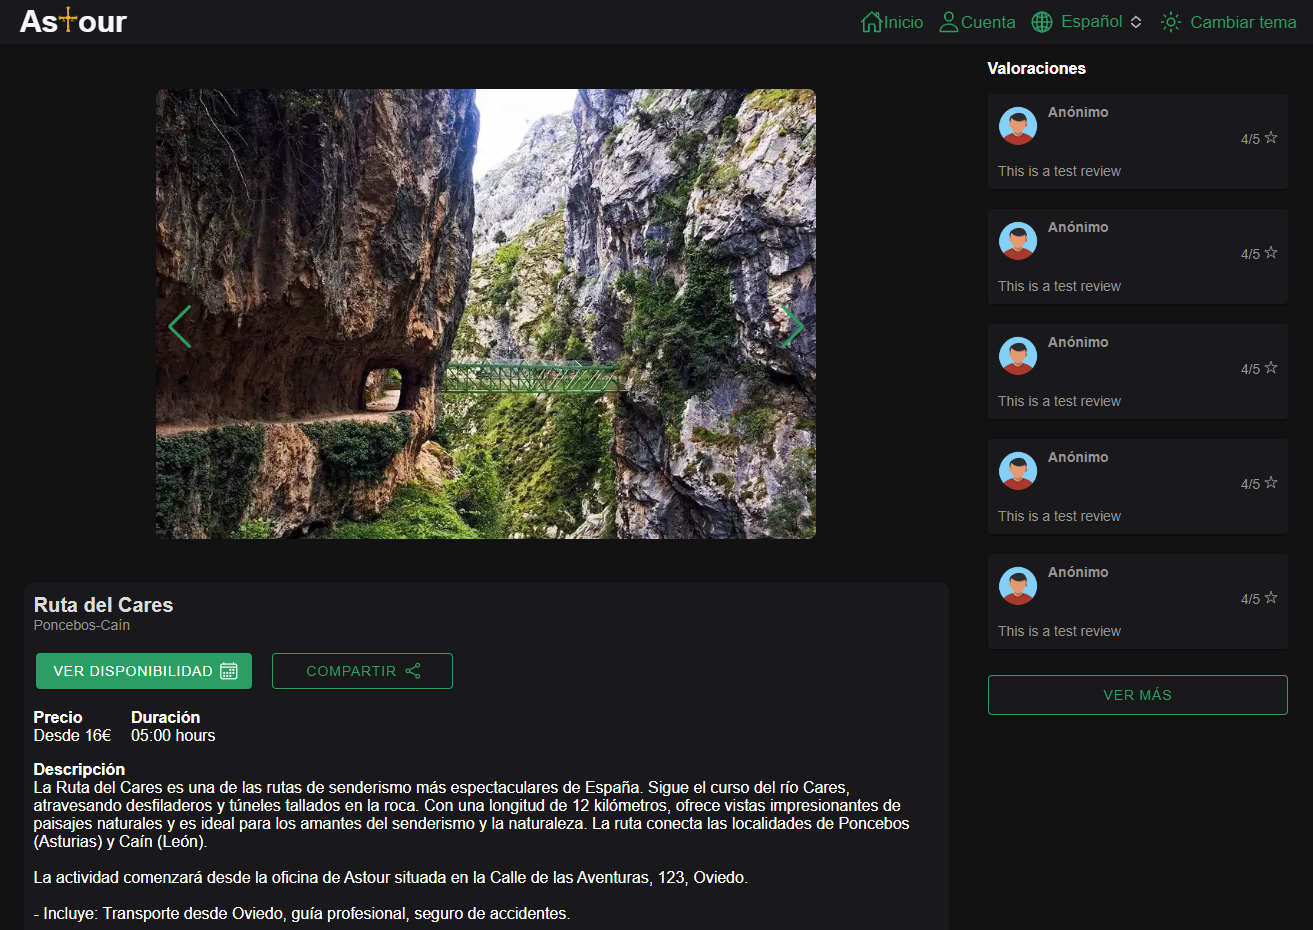
\includegraphics[width=1\textwidth]{7-Construccion/Manuales/web/detalles actividad.png}
		\caption{Exploración de Actividades \\ Detalles de la actividad}
		\label{fig:detalles-actividad}
	\end{minipage}
	\hfill
	\begin{minipage}{0.45\textwidth}
		\centering
		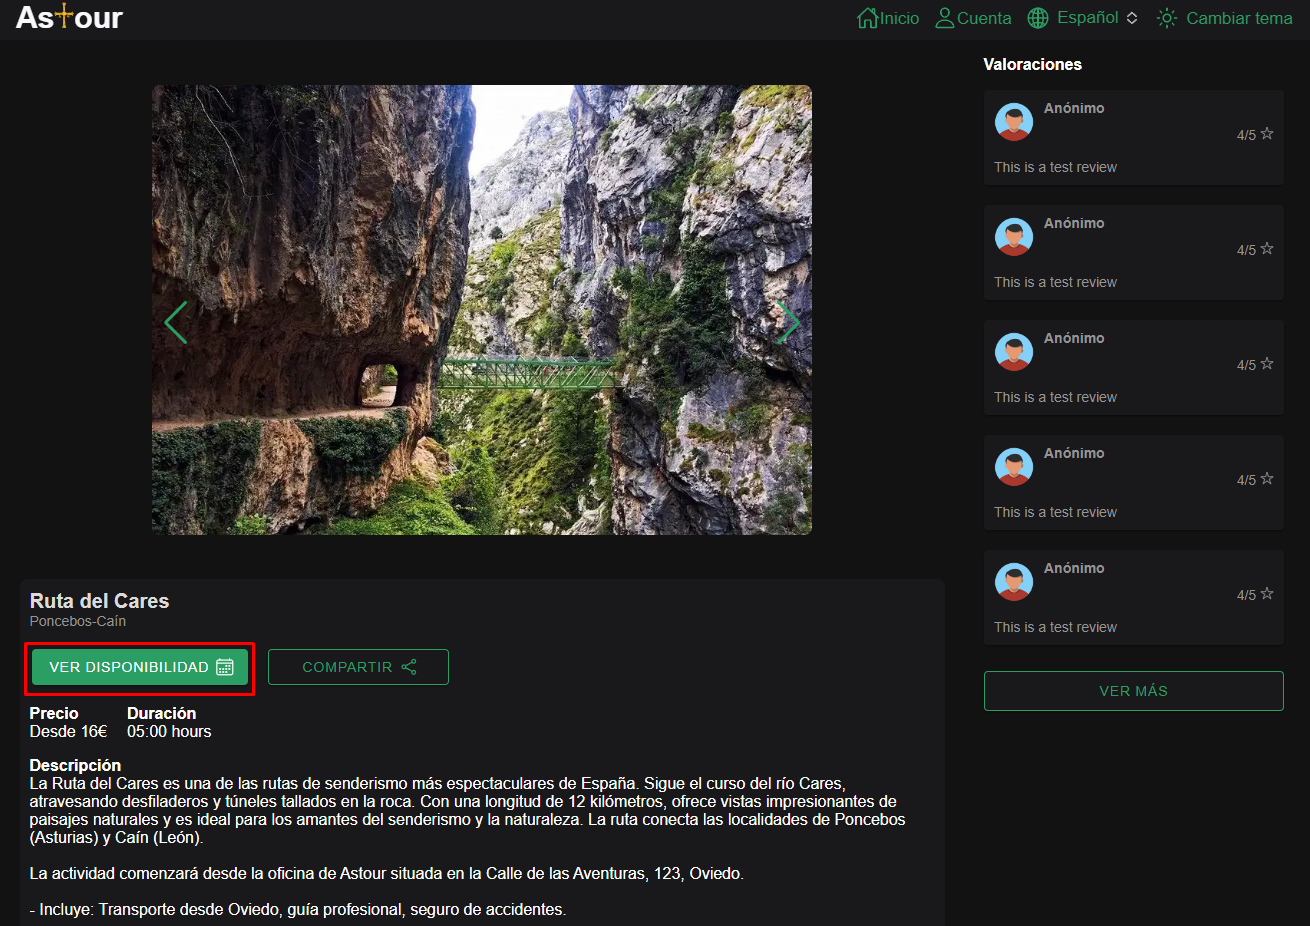
\includegraphics[width=1\textwidth]{7-Construccion/Manuales/web/ver disponibilidad.png}
		\caption{Exploración de Actividades \\ Ver disponibilidad}
		\label{fig:ver-disponibilidad}
	\end{minipage}
\end{figure}

\begin{figure}[H]
	\centering
	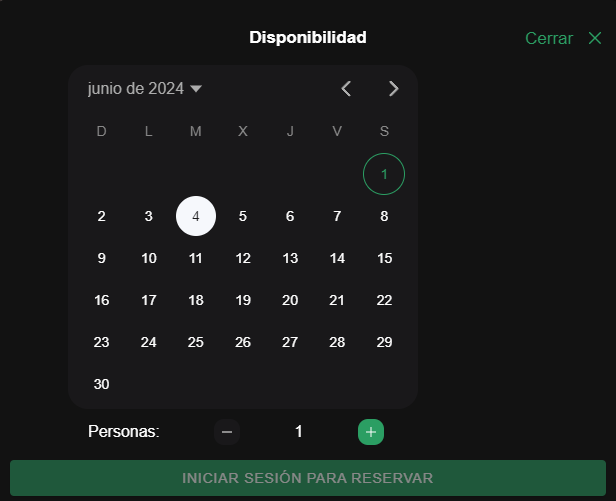
\includegraphics[width=0.4\textwidth]{7-Construccion/Manuales/web/disponibilidad sin.png}
	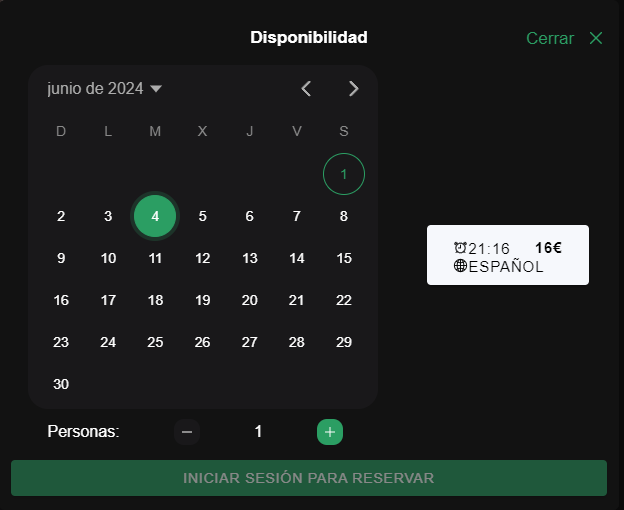
\includegraphics[width=0.4\textwidth]{7-Construccion/Manuales/web/disponibilidad selec dia.png}
	\caption{Exploración de Actividades \\ Calendario de disponibilidad}
	\label{fig:disponibilidad}
\end{figure}

\subsubsection{Cambiar Datos Personales}
Para cambiar tus datos personales, una vez hayas iniciado sesión, sigue estos pasos:
\begin{enumerate}
	\item Accede al apartado “Área personal” . Mira figuras \ref{fig:areaPersonal-movil}, \ref{fig:areaPersonal-app}, \ref{fig:areaPersonal-web}.

	\item Se abrirá una página con tus datos personales y varios botones de acción. Pulsa el botón “Editar perfil” para acceder al formulario de edición de datos personales.
	      Mirar figura \ref{fig:areaPersonal-editar}.
	\item Completa el formulario con los nuevos datos y pulsar el botón “Guardar cambios” para enviar el formulario.
	\item Si se quiere cambiar la contraseña habrá que pulsar el botón “Cambiar contraseña” para acceder al formulario de cambio de contraseña, completa el formulario con los nuevos datos y pulsa el botón “Guardar cambios” para enviar el formulario.
	      En versión móvil será necesario pulsar la pestaña “Cuenta” para acceder a la opción de cambiar la contraseña. Mirar figura \ref{fig:areaPersonal-cuenta-movil} y \ref{fig:areaPersonal-cambiar-contraseña}.
	\item En el caso de querer eliminar la cuenta habrá que pulsar el botón “Eliminar cuenta” para acceder a la ventana de confirmación de la eliminación de la cuenta. Toca el botón “Confirmar” para eliminar tu cuenta.
	      En versión móvil será necesario pulsar la pestaña “Cuenta” para acceder a la opción de eliminar la cuenta. Mirar figura \ref{fig:areaPersonal-cuenta-movil} y \ref{fig:areaPersonal-eliminar}.
\end{enumerate}

\begin{figure}[H]
	\centering
	\begin{minipage}{0.45\textwidth}
		\centering
		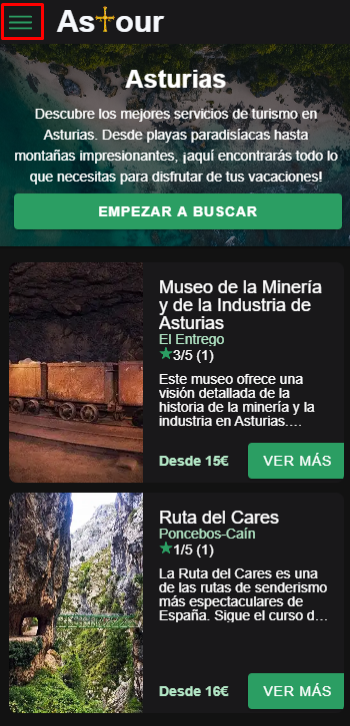
\includegraphics[width=0.3\textwidth]{7-Construccion/Manuales/mobile/menu marcado.png}
		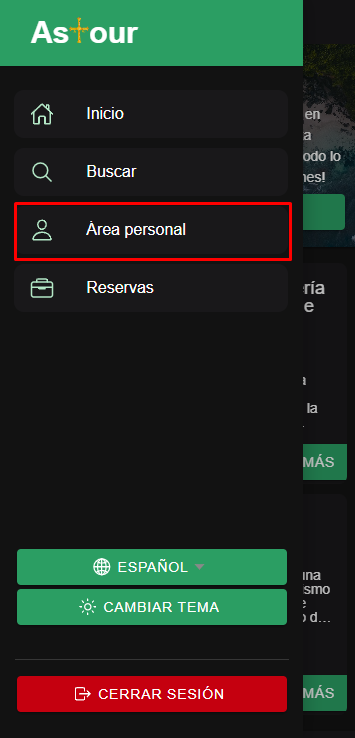
\includegraphics[width=0.3\textwidth]{7-Construccion/Manuales/mobile/area personal marcado.png}
		\caption{Perfil \\ Despliegue del menú y selección de la opción “Área personal” .}
		\label{fig:areaPersonal-movil}
	\end{minipage}
	\hfill
	\begin{minipage}{0.45\textwidth}
		\centering
		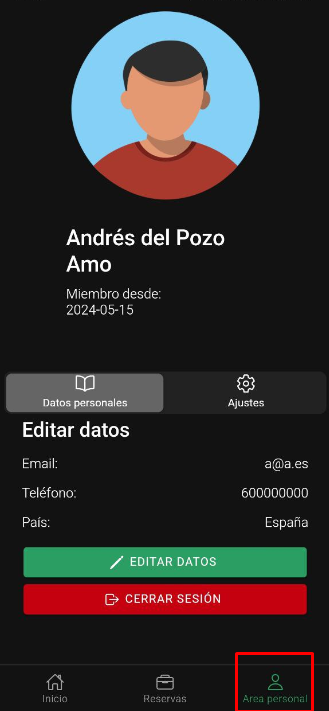
\includegraphics[width=0.3\textwidth]{7-Construccion/Manuales/app/P1-Perfil.png}
		\caption{Perfil \\ Selección de la opción “Perfil” de la barra inferior de navegación.}
		\label{fig:areaPersonal-app}
	\end{minipage}
\end{figure}

\begin{figure}[H]
	\centering
	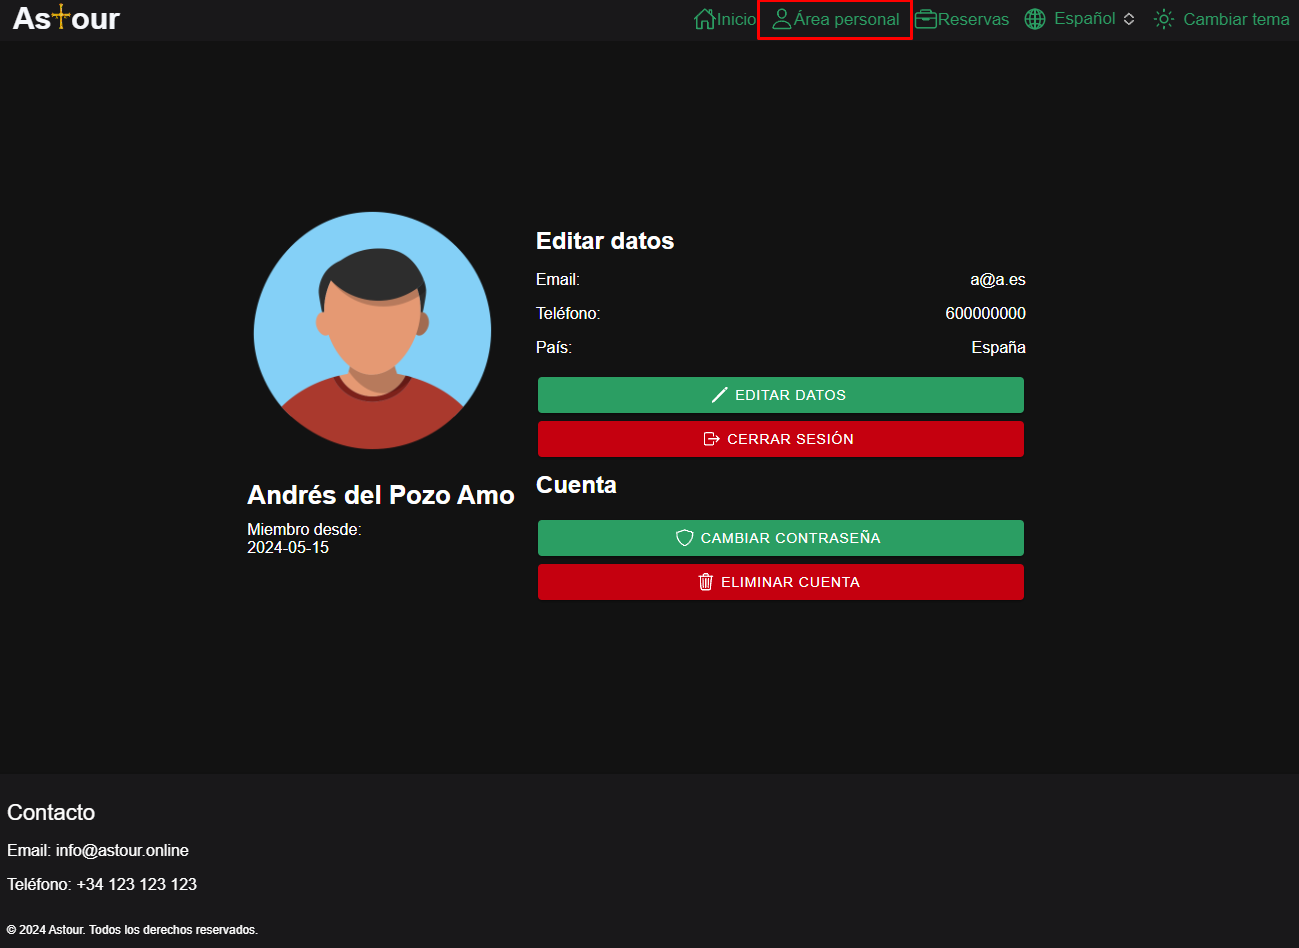
\includegraphics[width=0.5\textwidth]{7-Construccion/Manuales/web/area personal opcion.png}
	\caption{Perfil \\ Selección de la opción “Área personal” de la barra superior de navegación.}
	\label{fig:areaPersonal-web}
\end{figure}

\begin{figure}[H]
	\centering
	\begin{minipage}{0.45\textwidth}
		\centering
		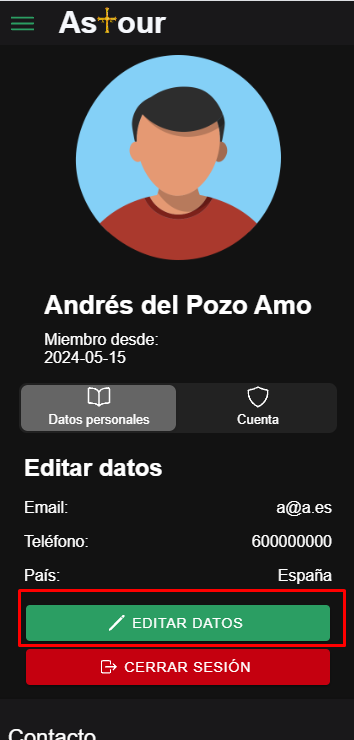
\includegraphics[width=0.3\textwidth]{7-Construccion/Manuales/mobile/editar datos.png}
		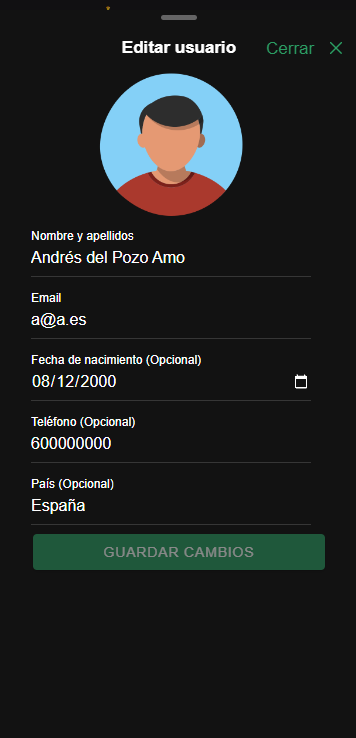
\includegraphics[width=0.3\textwidth]{7-Construccion/Manuales/mobile/formulario perfil.png}
		\caption{Perfil \\ Edición de datos personales.}
		\label{fig:areaPersonal-editar}
	\end{minipage}
	\hfill
	\begin{minipage}{0.45\textwidth}
		\centering
		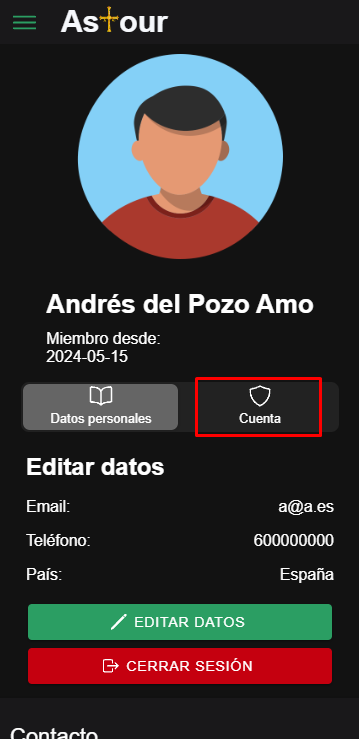
\includegraphics[width=0.3\textwidth]{7-Construccion/Manuales/mobile/apartado cuenta seleccionado.png}
		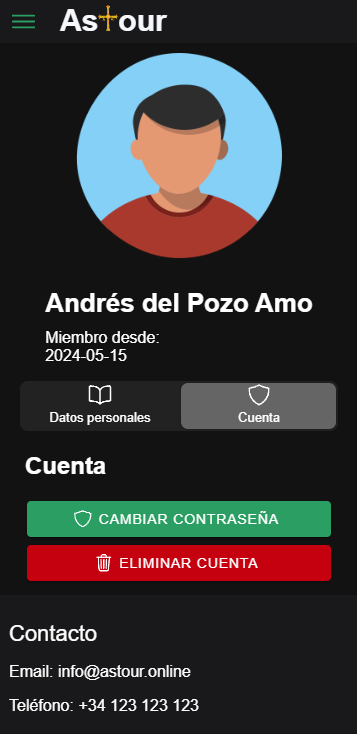
\includegraphics[width=0.3\textwidth]{7-Construccion/Manuales/mobile/editar cuenta.png}
		\caption{Perfil \\ Apartado cuenta}
		\label{fig:areaPersonal-cuenta-movil}
	\end{minipage}
\end{figure}

\begin{figure}[H]
	\centering
	\begin{minipage}{0.45\textwidth}
		\centering
		\includegraphics[width=0.3\textwidth]{7-Construccion/Manuales/mobile/cambiar contraseña.png}
		\includegraphics[width=0.3\textwidth]{7-Construccion/Manuales/mobile/formulario contraseña.png}
		\caption{Perfil \\ Cambio de contraseña}
		\label{fig:areaPersonal-cambiar-contraseña}
	\end{minipage}
	\hfill
	\begin{minipage}{0.45\textwidth}
		\centering
		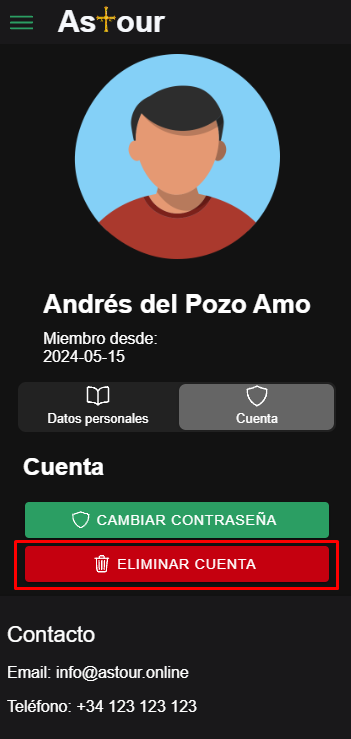
\includegraphics[width=0.3\textwidth]{7-Construccion/Manuales/mobile/eliminar cuenta.png}
		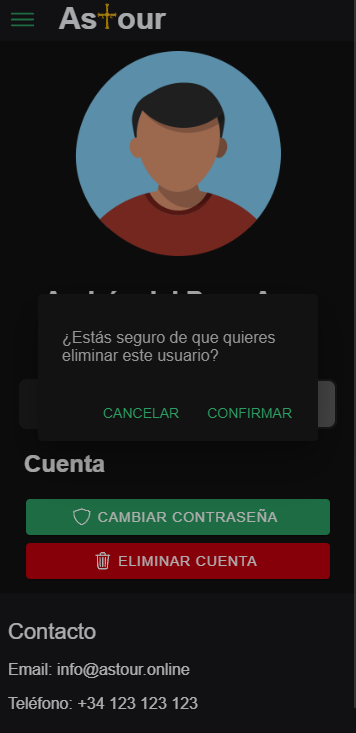
\includegraphics[width=0.3\textwidth]{7-Construccion/Manuales/mobile/confirmar eliminacion cuenta.png}
		\caption{Perfil \\ Eliminar cuenta}
		\label{fig:areaPersonal-eliminar}
	\end{minipage}
\end{figure}


\subsubsection{Cerrar Sesión}
Para poder cerrar sesión debes estar previamente logueado en la aplicación. Si no lo estás deberás hacerlo siguiendo los pasos descritos en la sección “Inicio de Sesión” .
\\ \\[1ex]
Para cerrar sesión debes buscar la opción “Cerrar sesión” . Mirar figuras \ref{fig:cuenta-movil}, \ref{fig:cuenta-app}, \ref{fig:cuenta-web}.
\\ \\[1ex]
Se te redirigirá a la página de inicio y habrás cerrado sesión con éxito. Si deseas volver a iniciar sesión, sigue los pasos descritos en la sección “Inicio de Sesión” .


\begin{figure}[H]
	\centering
	\begin{minipage}{0.45\textwidth}
		\centering
		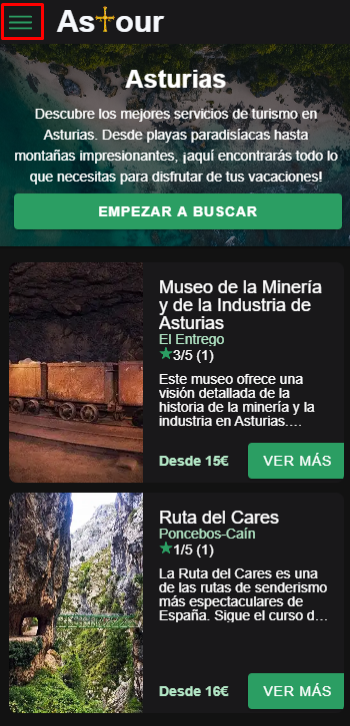
\includegraphics[width=0.3\textwidth]{7-Construccion/Manuales/mobile/menu marcado.png}
		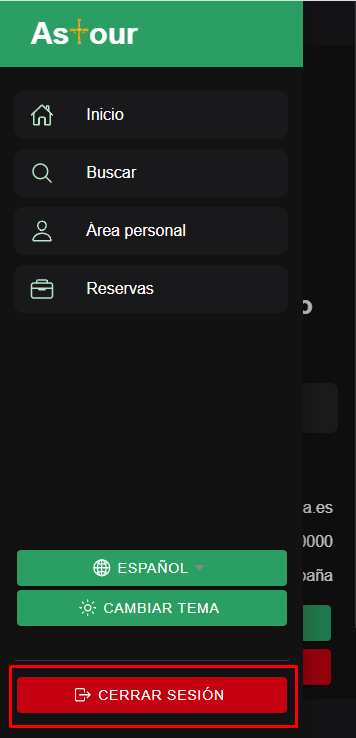
\includegraphics[width=0.3\textwidth]{7-Construccion/Manuales/mobile/cerrar sesion marcado.png}
		\caption{Cerrar sesión - Despliegue del menú y selección de la opción “Cerrar sesión” .}
		\label{fig:cuenta-movil}
	\end{minipage}
	\hfill
	\begin{minipage}{0.45\textwidth}
		\centering
		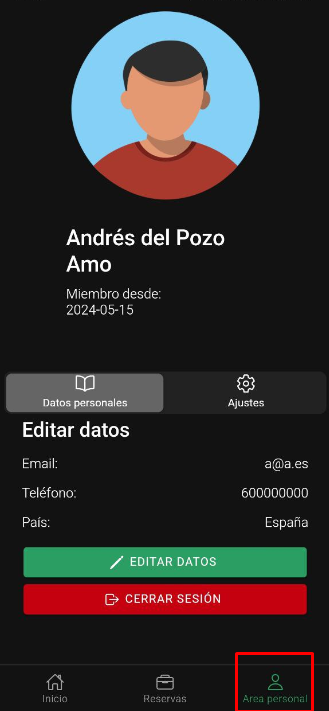
\includegraphics[width=0.3\textwidth]{7-Construccion/Manuales/app/P1-Perfil.png}
		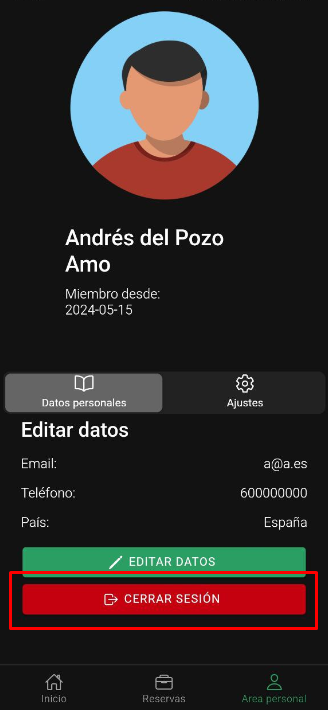
\includegraphics[width=0.3\textwidth]{7-Construccion/Manuales/app/P2-CerrarSesion.png}
		\caption{Cerrar sesión - Cerrar sesión desde la app.}
		\label{fig:cuenta-app}
	\end{minipage}
\end{figure}

\begin{figure}[H]
	\centering
	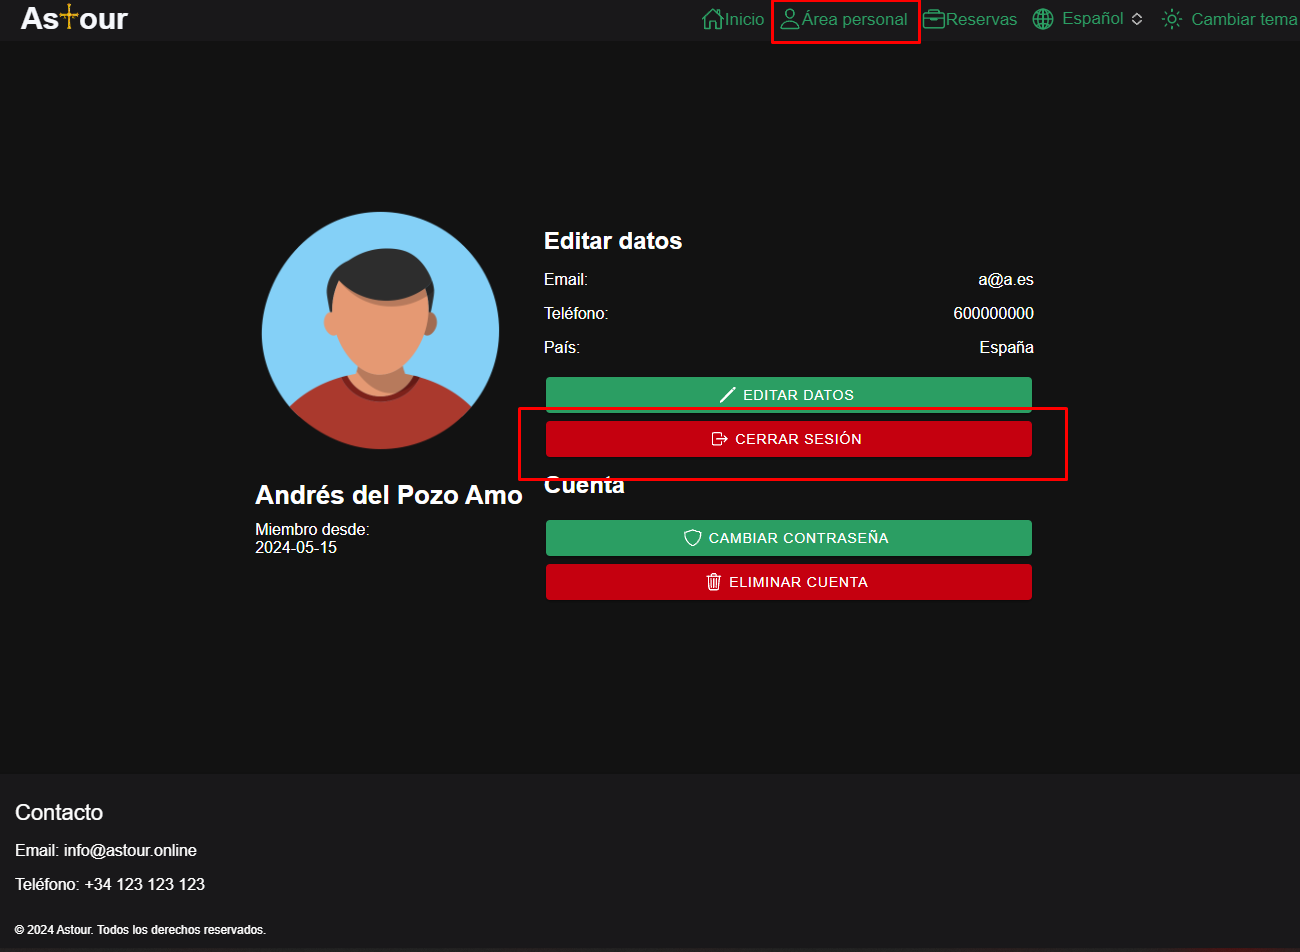
\includegraphics[width=0.5\textwidth]{7-Construccion/Manuales/web/cerrar sesion.png}
	\caption{Cerrar sesión - Cerrar sesión desde la web.}
	\label{fig:cuenta-web}
\end{figure}

\subsubsection{Cambiar Idioma}
Para cambiar el idioma de la página sigue estos pasos:
\begin{enumerate}
	\item Busca el botón “Español” . El contenido del botón puede variar dependiendo del idioma actual. Mirar figura \ref{fig:idioma-movil}, \ref{fig:idioma-app}, \ref{fig:idioma-web}.

	\item Se abrirá un menú desplegable con una lista de idiomas disponibles. Toca el idioma deseado para cambiar el idioma de la aplicación.
	      El contenido de la aplicación se actualizará automáticamente con el idioma seleccionado. Mirar figura \ref{fig:cambio-idioma}.

\end{enumerate}

\begin{figure}[H]
	\centering
	\begin{minipage}{0.45\textwidth}
		\centering
		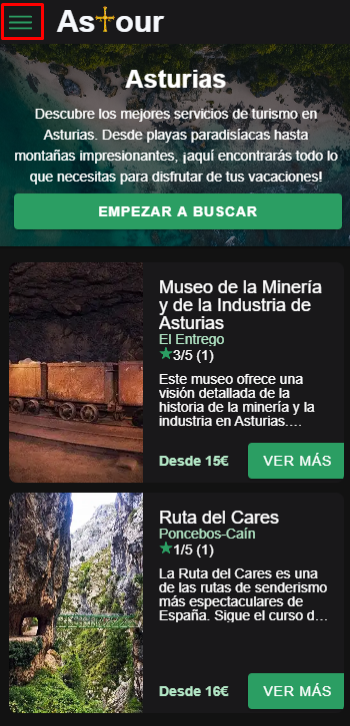
\includegraphics[width=0.3\textwidth]{7-Construccion/Manuales/mobile/menu marcado.png}
		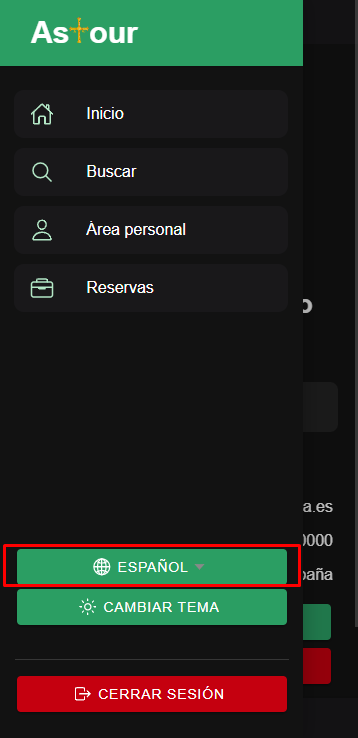
\includegraphics[width=0.3\textwidth]{7-Construccion/Manuales/mobile/idioma marcado.png}
		\caption{Cambiar idioma - Despliegue del menú y selección de la opción “Español” .}
		\label{fig:idioma-movil}
	\end{minipage}
	\hfill
	\begin{minipage}{0.45\textwidth}
		\centering
		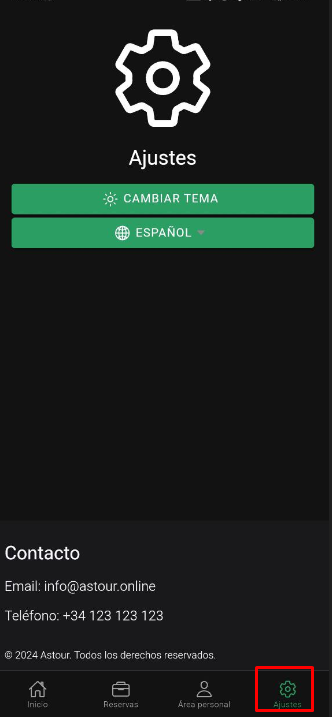
\includegraphics[width=0.3\textwidth]{7-Construccion/Manuales/app/P1-Configuration.png}
		\caption {Cambiar idioma - Ir a los ajustes.}
		\label{fig:idioma-app}
	\end{minipage}
\end{figure}

\begin{figure}[H]
	\centering
	\begin{minipage}{0.45\textwidth}
		\centering
		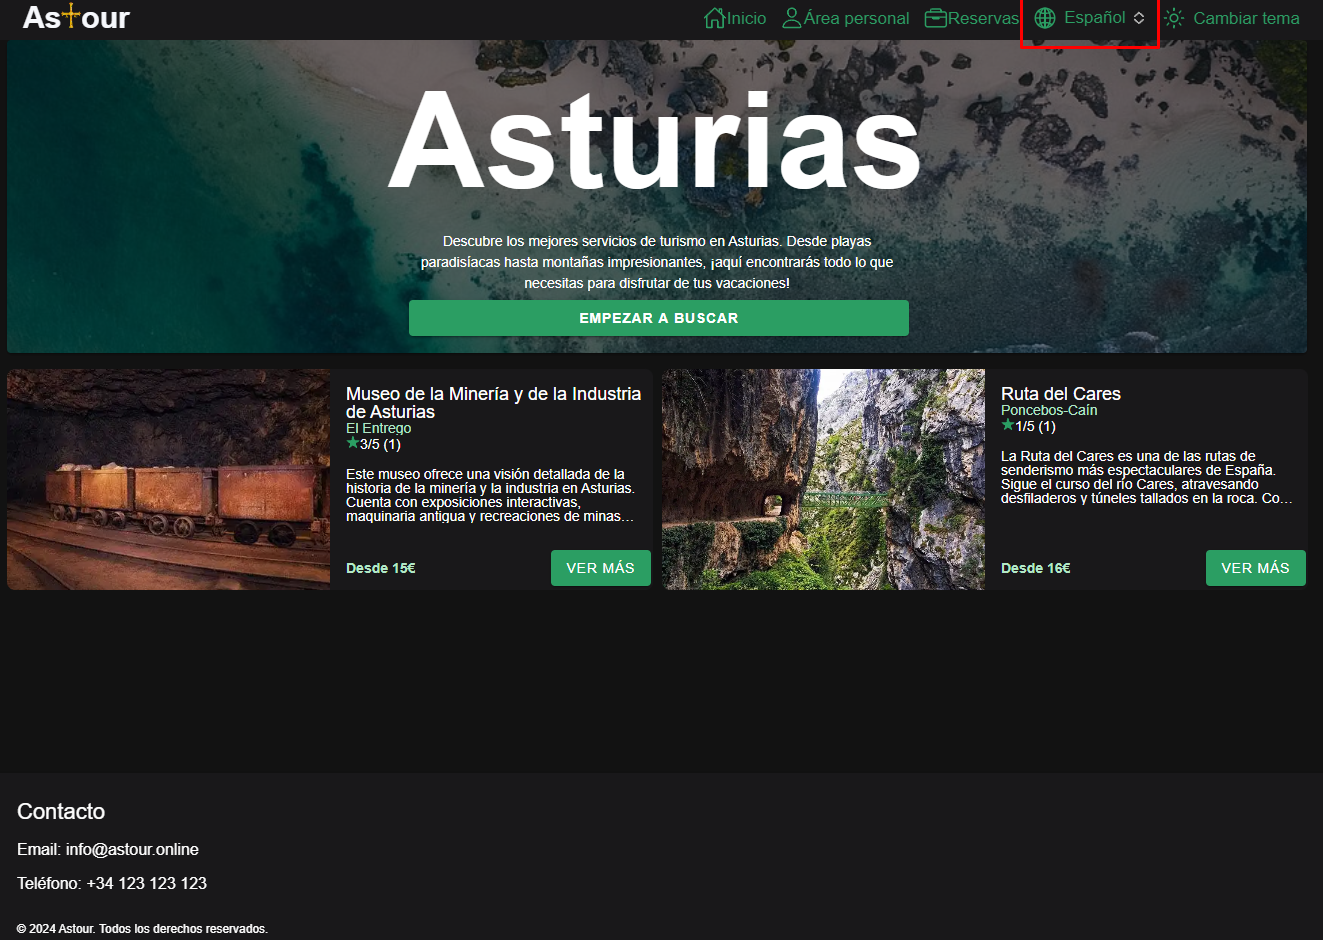
\includegraphics[width=1\textwidth]{7-Construccion/Manuales/web/idioma.png}
		\caption{Cambiar idioma - Cambio de idioma.}
		\label{fig:idioma-web}
	\end{minipage}
	\begin{minipage}{0.45\textwidth}
		\centering
		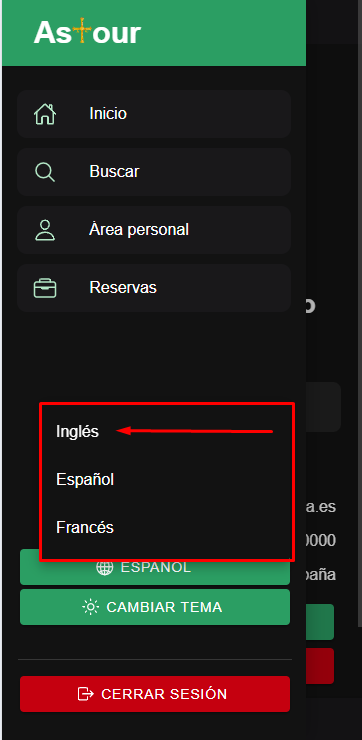
\includegraphics[width=0.3\textwidth]{7-Construccion/Manuales/mobile/opciones idioma.png}
		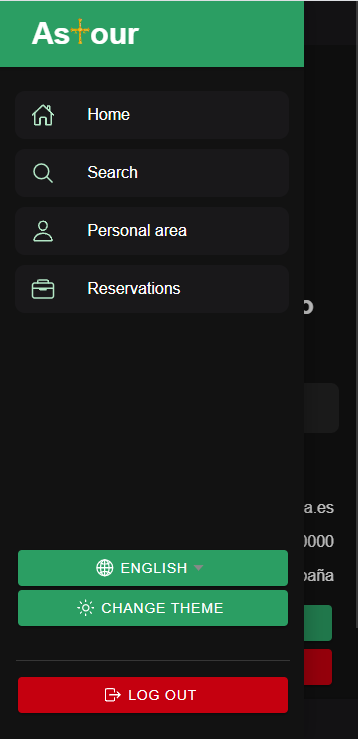
\includegraphics[width=0.3\textwidth]{7-Construccion/Manuales/mobile/ingles.png}
		\caption{Cambiar idioma - Cambio de idioma.}
		\label{fig:cambio-idioma}
	\end{minipage}
\end{figure}

\subsubsection{Cambiar Tema}
\begin{enumerate}
	\item Busca el botón “Cambiar tema” . Mirar figura \ref{fig:tema-movil}, \ref{fig:tema-app}, \ref{fig:tema-web}.

	\item La página web se actualizará automáticamente con el tema contrario. Si el tema actual es claro, se cambiará a oscuro y viceversa.
	      El icono de la opción de tema cambiará al tema contrario. Si el tema actual es claro, se cambiará a una luna y si el tema actual es oscuro, se cambiará a un sol.
	      Mirar figura \ref{fig:cambio-tema}.

\end{enumerate}

\begin{figure}[H]
	\centering
	\begin{minipage}{0.45\textwidth}
		\centering
		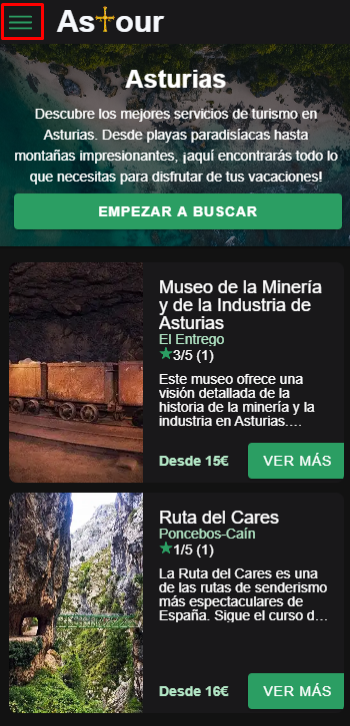
\includegraphics[width=0.3\textwidth]{7-Construccion/Manuales/mobile/menu marcado.png}
		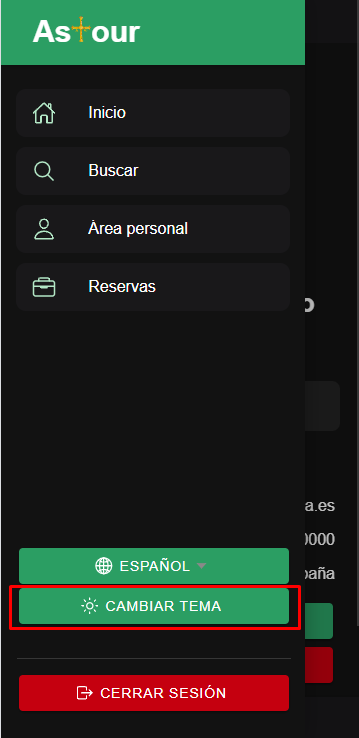
\includegraphics[width=0.3\textwidth]{7-Construccion/Manuales/mobile/tema marcado.png}
		\caption{Cambiar tema - Despliegue del menú y selección de la opción “Cambiar tema” .}
		\label{fig:tema-movil}
	\end{minipage}
	\hfill
	\begin{minipage}{0.45\textwidth}
		\centering
		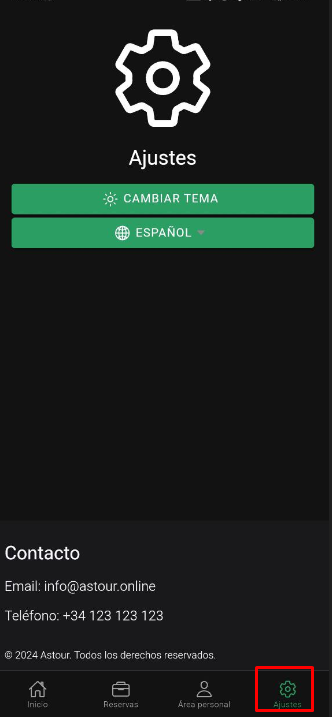
\includegraphics[width=0.3\textwidth]{7-Construccion/Manuales/app/P1-Configuration.png}
		\caption{Cambiar tema - Ir a los ajustes.}
		\label{fig:tema-app}
	\end{minipage}
\end{figure}

\begin{figure}[H]
	\centering
	\begin{minipage}{0.45\textwidth}
		\centering
		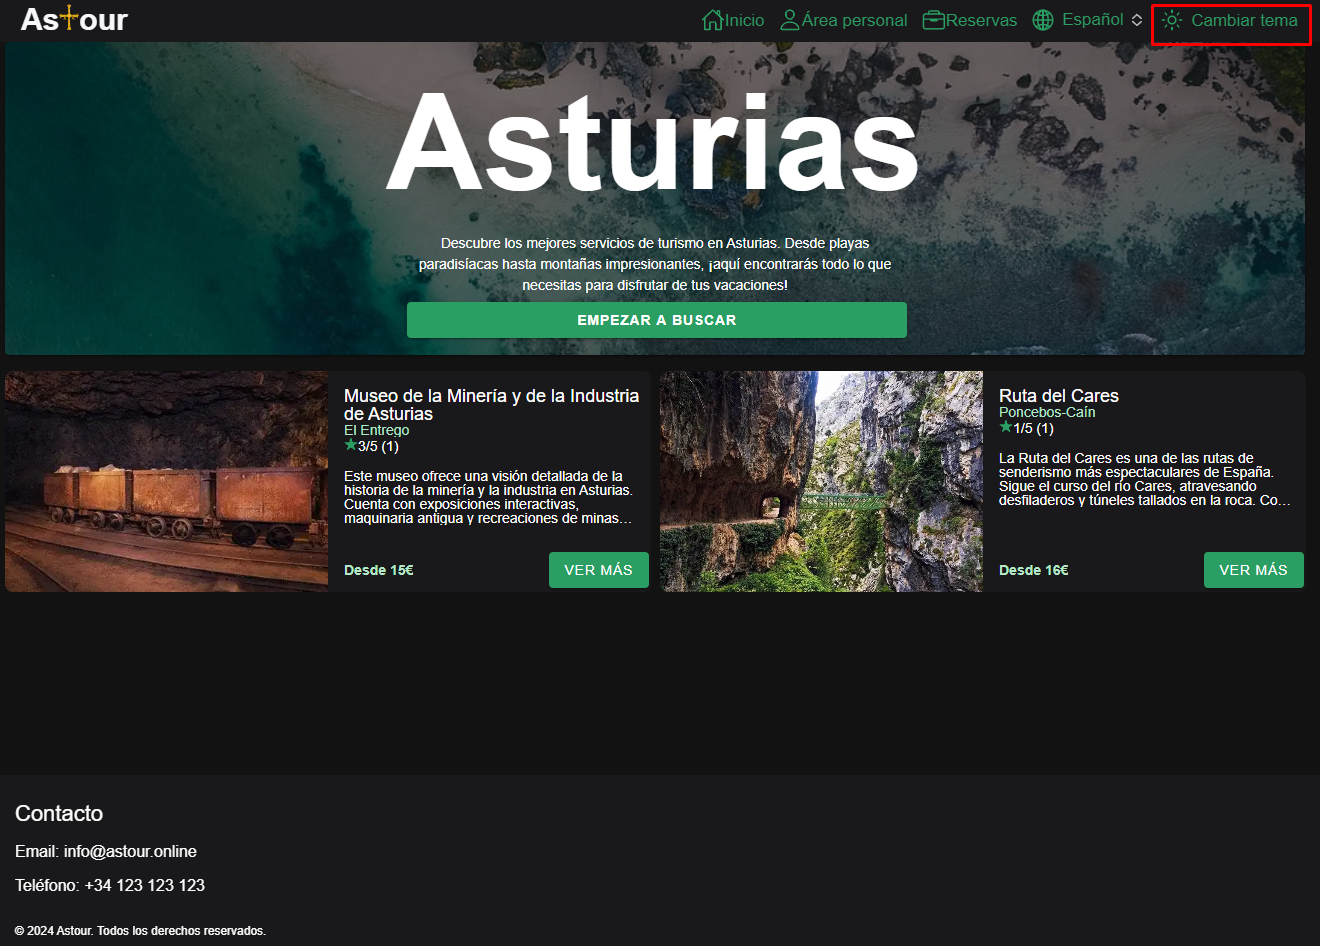
\includegraphics[width=1\textwidth]{7-Construccion/Manuales/web/tema.png}
		\caption{Cambiar tema - Cambio de tema.}
		\label{fig:tema-web}
	\end{minipage}
	\hfill
	\begin{minipage}{0.45\textwidth}
		\centering
		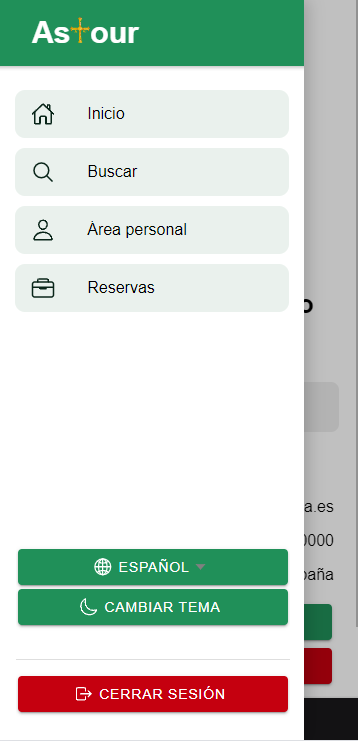
\includegraphics[width=0.3\textwidth]{7-Construccion/Manuales/mobile/tema claro.png}
		\caption{Cambiar tema - Cambio de tema.}
		\label{fig:cambio-tema}
	\end{minipage}
\end{figure}

\subsubsection{Soporte Técnico}
Si encuentras algún problema o tienes alguna pregunta relacionada con el uso de nuestra aplicación, no dudes en contactar a nuestro equipo de soporte técnico.
Puedes encontrar la información de contacto en el apartado “Contacto” de la parte inferior de la página o en el apartado ajustes de la app. Mirar figuras \ref{fig:contacto-movil}, \ref{fig:contacto-app}.
\begin{figure}[H]
	\centering
	\begin{minipage}{0.45\textwidth}
		\centering
		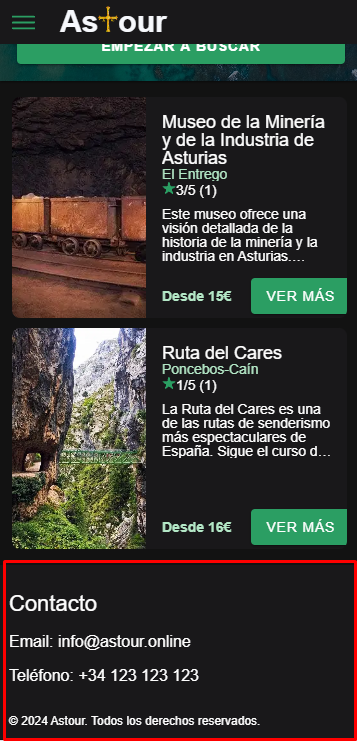
\includegraphics[width=0.3\textwidth]{7-Construccion/Manuales/mobile/contacto.png}
		\caption{Contacto - Información de contacto en la web}
		\label{fig:contacto-movil}
	\end{minipage}
	\hfill
	\begin{minipage}{0.45\textwidth}
		\centering
		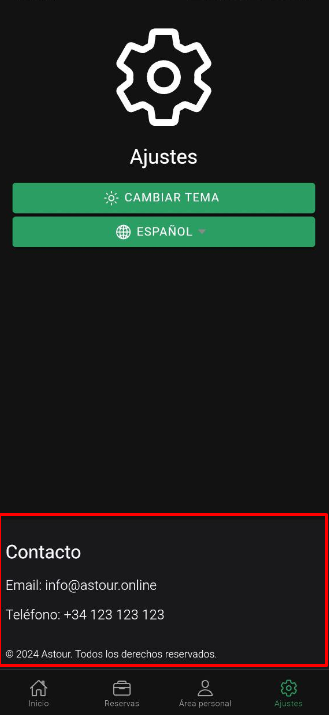
\includegraphics[width=0.3\textwidth]{7-Construccion/Manuales/app/soporte.png}
		\caption{Contacto - Información de contacto en la app}
		\label{fig:contacto-app}
	\end{minipage}
\end{figure}

\newpage
\subsubsection{Funciones como Turistas}
\hrulefill

\subsubsection{Reservar una Actividad}
Para reservar una actividad sigue estos pasos:

\begin{enumerate}
	\item Siga las indicaciones de la sección “Exploración de Actividades” para encontrar la actividad deseada y ver la información detallada de la misma.

	\item Selecciona el horario y el idioma deseados dentro de las opciones disponibles y pulsa el botón “Reservar” para empezar la reserva. Mirar figura \ref{fig:disponibilidad-reservar}.
	      Si no has iniciado sesión, se te pedirá que inicies sesión o te registres. Sigue las indicaciones de la sección “Autenticación” para iniciar sesión o registrarte.
	      Se te llevará a una página de confirmación de la reserva, donde verás tus datos personales (se pueden modificar si es necesario), el precio total y un formulario para introducir los datos de pago. Mirar figu \ref{fig:formulario-reservar}.

	\item Completa el formulario con los datos de pago y pulsa el botón “Pagar” para finalizar la reserva.
	      Si la reserva se realiza desde la app móvil, el fomulario de pago se abrirá en un modal al presionar el botón “Pagar” . Mirar figura \ref{fig:formulario-app-reservar}.
	      Se te mostrará una ventana de confirmación de la reserva. Mirar figura \ref{fig:confirmacion-reserva}.

\end{enumerate}

\begin{figure}[H]
	\centering
	\begin{minipage}{0.45\textwidth}
		\centering
		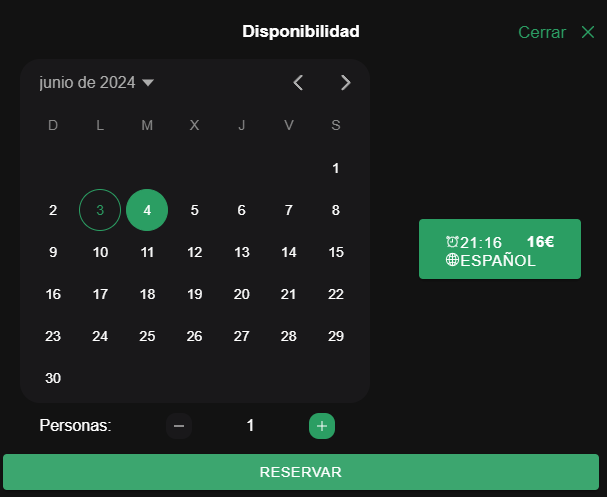
\includegraphics[width=0.8\textwidth]{7-Construccion/Manuales/web/disponibilidad reservar.png}
		\caption{Reservar una actividad \\ Selección de horario e idioma y formulario de reserva.}
		\label{fig:disponibilidad-reservar}
	\end{minipage}
	\hfill
	\begin{minipage}{0.45\textwidth}
		\centering
		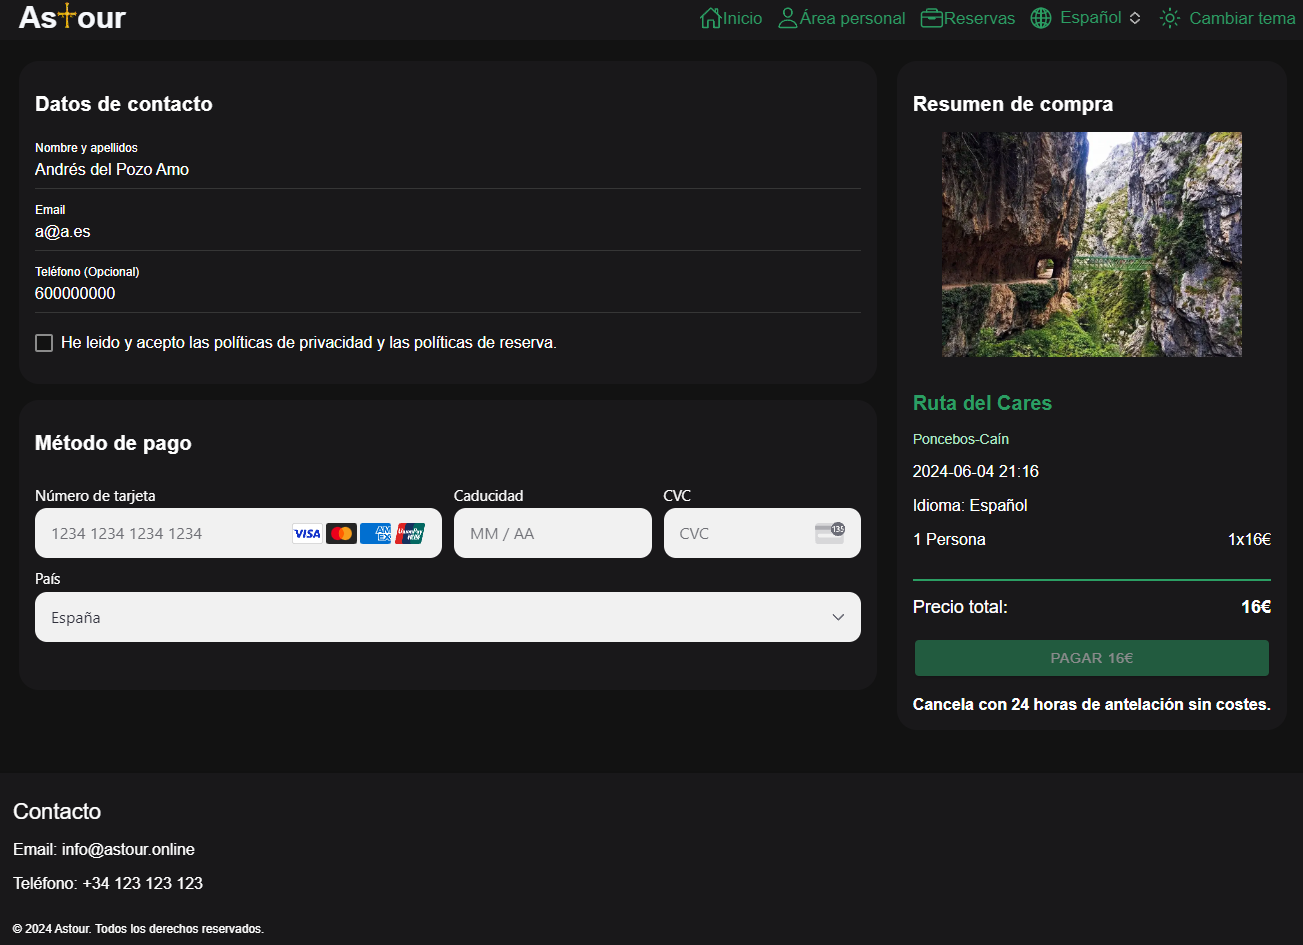
\includegraphics[width=0.9\textwidth]{7-Construccion/Manuales/web/formulario-reservar.png}
		\caption{Reservar una actividad \\ Formulario de reserva.}
		\label{fig:formulario-reservar}
	\end{minipage}
\end{figure}

\begin{figure}[H]
	\centering
	\begin{minipage}{0.45\textwidth}
		\centering
		\includegraphics[width=0.35\textwidth]{7-Construccion/Manuales/app/P2-Reservar.png}
		\includegraphics[width=0.35\textwidth]{7-Construccion/Manuales/app/P3-Reservar.png}
		\caption{Reservar una actividad \\ Formulario de reserva en la app.}
		\label{fig:formulario-app-reservar}
	\end{minipage}
	\hfill
	\begin{minipage}{0.45\textwidth}
		\centering
		\includegraphics[width=1\textwidth]{7-Construccion/Manuales/web/thankYou.png}
		\caption{Reservar una actividad \\ Confirmación de la reserva.}
		\label{fig:confirmacion-reserva}
	\end{minipage}
\end{figure}


\subsubsection{Gestión de Reservas}
Para gestionar tus reservas sigue estos pasos:
\begin{enumerate}
	\item Accede al apartado “Reservas” . Mirar figuras \ref{fig:opcion-mobile-reservas}, \ref{fig:opcion-app-reservas}, \ref{fig:opcion-web-reservas}.

	\item Se abrirá una página con un listado de tus reservas activas y pasadas.
	      Para ver más detalles de una reserva, pulsa el botón “Gestionar” de la reserva deseada.
	      Se abrirá una nueva ventana con la información detallada de la reserva, incluyendo la actividad, la fecha y hora, el idioma, el número de personas y el precio total.
	      Mirar figura \ref{fig:detalles-reserva}.

	\item Para cancelar una reserva, pulsa el botón “Cancelar” de la reserva deseada y se abrirá una ventana de confirmación de la cancelación.
	      Toca el botón “Confirmar” para cancelar la reserva. Mirar figura \ref{fig:cancelar-reserva}.

\end{enumerate}

\begin{figure}[H]
	\centering
	\begin{minipage}{0.45\textwidth}
		\centering
		\includegraphics[width=0.3\textwidth]{7-Construccion/Manuales/mobile/menu marcado.png}
		\includegraphics[width=0.3\textwidth]{7-Construccion/Manuales/mobile/reservas marcado.png}
		\caption{Gestión de reservas \\ Despliegue del menú y selección de la opción “Reservas” .}
		\label{fig:opcion-mobile-reservas}
	\end{minipage}
	\hfill
	\begin{minipage}{0.45\textwidth}
		\centering
		\includegraphics[width=0.3\textwidth]{7-Construccion/Manuales/app/P1-GestionReserva.png}
		\caption{Gestión de reservas \\ Selección de la opción “Reservas” de la barra inferior de navegación.}
		\label{fig:opcion-app-reservas}
	\end{minipage}
\end{figure}

\begin{figure}[H]
	\begin{minipage}{0.40\textwidth}
		\centering
		\includegraphics[width=1\textwidth]{7-Construccion/Manuales/web/reservas opcion.png}
		\caption{Gestión de reservas \\ Selección de la opción “Reservas” de la barra superior de navegación.}
		\label{fig:opcion-web-reservas}
	\end{minipage}
	\hfill
	\begin{minipage}{0.5\textwidth}
		\centering
		\includegraphics[width=0.3\textwidth]{7-Construccion/Manuales/mobile/gestionar.png}
		\includegraphics[width=0.65\textwidth]{7-Construccion/Manuales/web/reserva detalles.png}
		\caption{Gestión de reservas \\ Redirección a la información detallada de la reserva.}
		\label{fig:detalles-reserva}
	\end{minipage}
\end{figure}

\begin{figure}[H]
	\centering
	\includegraphics[width=0.2\textwidth]{7-Construccion/Manuales/mobile/cancelar reserva.png}
	\includegraphics[width=0.2\textwidth]{7-Construccion/Manuales/mobile/confirmar cancelacion reserva.png}
	\caption{Gestión de reservas \\ Cancelar reserva.}
	\label{fig:cancelar-reserva}
\end{figure}

\subsubsection{Publicar una Valoración}
Recuerda que puedes publicar una valoración de una actividad después de haberla realizado.

Para publicar una valoración de una actividad desde tu dispositivo móvil, sigue estos pasos:
\begin{enumerate}
	\item Accede al apartado “Reservas” . Mirar figuras \ref{fig:opcion-mobile-reservas}, \ref{fig:opcion-app-reservas}, \ref{fig:opcion-web-reservas}.

	\item Se abrirá una página con un listado de tus reservas activas y pasadas. Toca el botón “Gestionar” de la reserva que deseas valorar.
	      Se abrirá una nueva ventana con la información detallada de la reserva, incluyendo la actividad, la fecha y hora, el idioma, el número de personas y el precio total.
	      Mirar figura \ref{fig:detalles-reserva-completada}.
	\item Para publicar una valoración, pulsa el botón “Añadir valoración” de la reserva deseada. Se abrirá una nueva ventana con un formulario para introducir tu puntuación y comentario (campo no obligatorio).
	      Mirar figura \ref{fig:modal-valoracion}.
	\item Completa el formulario y pulsa el botón “Guardar cambios” para enviar la valoración.
\end{enumerate}

\begin{figure}[H]
	\centering
	\begin{minipage}{0.45\textwidth}
		\centering
		\includegraphics[width=0.3\textwidth]{7-Construccion/Manuales/mobile/gestionar completada.png}
		\includegraphics[width=0.65\textwidth]{7-Construccion/Manuales/web/reserva detalles completada.png}
		\caption{Gestión de reservas \\ Redirección a la información detallada de la reserva.}
		\label{fig:detalles-reserva-completada}
	\end{minipage}
	\hfill
	\begin{minipage}{0.45\textwidth}
		\centering
		\includegraphics[width=0.3\textwidth]{7-Construccion/Manuales/mobile/añadir valoracion.png}
		\includegraphics[width=0.3\textwidth]{7-Construccion/Manuales/mobile/formulario valoracion.png}
		\caption{Gestión de reservas \\ Formulario valoración}
		\label{fig:modal-valoracion}
	\end{minipage}
\end{figure}

\newpage
\subsubsection{Funciones como Administrador}
\hrulefill

\subsubsection{Panel de contol}
Una vez has iniciado sesión, podrás acceder a tu panel de control haciendo clic en la opción “Panel de control” del menú superior de la página de inicio. Mirar figura \ref{fig:panel-control-opcion}.
En tu panel de control, podrás ver estadísticas sobre las reservas realizadas, los beneficios obtenidos, el número de usuarios registrados, reservas recientes y gráficos informativos. Mirar figura \ref{fig:panel-control}.

En esta página también se podrá ir a la sección de usuarios y actividades para poder gestionarlos.

\begin{figure}[H]
	\centering
	\begin{minipage}{0.45\textwidth}
		\centering
		\includegraphics[width=1\textwidth]{7-Construccion/Manuales/web/panel control opcion.png}
		\caption{Dashboard \\ Opción de panel de control}
		\label{fig:panel-control-opcion}
	\end{minipage}
	\hfill
	\begin{minipage}{0.45\textwidth}
		\centering
		\includegraphics[width=1\textwidth]{7-Construccion/Manuales/web/panel control.png}
		\caption{Dashboard \\ Estadísticas del panel de control}
		\label{fig:panel-control}
	\end{minipage}
\end{figure}

\subsubsection{Gestión de usuarios}
Para gestionar los usuarios, una vez has iniciado sesión, sigue estos pasos:
\begin{enumerate}
	\item Haz clic en la opción “Panel de control” del menú superior de la página de inicio. Mirar figura \ref{fig:panel-control-opcion}.
	\item Se abrirá una página con estadísticas y un menú en la parte izquierda. Mirar figura \ref{fig:panel-control}.
	\item Haz clic en la opción “Usuarios” del menú, para acceder a la lista de usuarios registrados. Mirar figura \ref{fig:usuarios-opcion}.
	\item Se pueden filtrar los usuarios por nombre, email o número de identificación, haciendo uso de la barra de búsqueda.
	\item Haz clic en el icono del ojo para acceder a la información detallada del usuario.
	\item Haz clic en el icono del lápiz para editar el usuario.
	\item Haz click en el icono de la papelera para eliminar el usuario de la aplicación.
	\item En la parte superior derecha de la lista de usuarios, se encuentra un botón para añadir un nuevo usuario. Mirar figura \ref{fig:usuarios-add}.
\end{enumerate}

\begin{figure}[H]
	\centering
	\begin{minipage}{0.45\textwidth}
		\centering
		\includegraphics[width=1\textwidth]{7-Construccion/Manuales/web/usuarios opcion.png}
		\caption{Dashboard \\ Opción de usuarios}
		\label{fig:usuarios-opcion}
	\end{minipage}
	\hfill
	\begin{minipage}{0.45\textwidth}
		\centering
		\includegraphics[width=1\textwidth]{7-Construccion/Manuales/web/usuario add.png}
		\caption{Dashboard \\ Añadir usuario}
		\label{fig:usuarios-add}
	\end{minipage}
\end{figure}

\subsubsection{Gestión de actividades}
Para gestionar las actividades, una vez has iniciado sesión, sigue estos pasos:
\begin{enumerate}
	\item Haz clic en la opción “Panel de control” del menú superior de la página de inicio. Mirar figura \ref{fig:panel-control-opcion}.
	\item Se abrirá una página con estadísticas y un menú en la parte izquierda. Mirar figura \ref{fig:panel-control}.
	\item Haz clic en la opción “Actividades” del menú, para acceder a la lista de actividades registradas. Mirar figura \ref{fig:actividades-opcion}.
	\item Se pueden filtrar las actividades por nombre o ubicación, haciendo uso de la barra de búsqueda.
	\item Haz clic en el icono del ojo para acceder a la información detallada de la actividad.
	\item Haz clic en el icono del lápiz para editar la actividad.
	\item Haz click en el icono de la papelera para eliminar la actividad de la aplicación y todos sus eventos asociados. Mirar figura \ref{fig:actividades-ver-eventos}.
	\item En el menú de la parte izquierda, se encuentra:
	      \begin{itemize}
		      \item un botón para activar o desactivar la visibilidad de los eventos de las actividades.
		      \item un rango de fechas para filtrar los eventos por fecha de inicio.
		      \item un campo para mostrar o ocultar los eventos cancelados.
		      \item un botón para añadir un nuevo evento al sistema.
	      \end{itemize}
	\item En la parte superior derecha de la lista de actividades, se encuentra un botón para añadir una nueva actividad. Mirar figura \ref{fig:actividades-add}.
\end{enumerate}

\begin{figure}[H]
	\centering
	\begin{minipage}{0.45\textwidth}
		\centering
		\includegraphics[width=1\textwidth]{7-Construccion/Manuales/web/actividades opcion.png}
		\caption{Dashboard \\ Opción de actividades}
		\label{fig:actividades-opcion}
	\end{minipage}
	\hfill
	\begin{minipage}{0.45\textwidth}
		\centering
		\includegraphics[width=1\textwidth]{7-Construccion/Manuales/web/actividades ver eventos.png}
		\caption{Dashboard \\ Ver eventos}
		\label{fig:actividades-ver-eventos}
	\end{minipage}
\end{figure}

\begin{figure}[H]
	\centering
	\includegraphics[width=0.5\textwidth]{7-Construccion/Manuales/web/actividad add.png}
	\caption{Dashboard \\ Añadir actividad}
	\label{fig:actividades-add}
\end{figure}

\newpage
\subsubsection{Funciones como Guía}
\hrulefill

\subsubsection{Ver eventos proximos}
Para ver los eventos que tendrás próximamente, deberás acceder a “Eventos próximos” . Mirar figuras \ref{fig:eventos-proximos-opcion-movil}, \ref{fig:eventos-proximos-opcion-app}, \ref{fig:eventos-proximos-opcion-web} .
Se abrirá una página donde podrás seleccionar la fecha deseada para ver los eventos programados para ese día.
Y se mostrará una lista con los eventos programados para la fecha seleccionada, incluyendo el nombre, la descripción, la duración, la ubicación, el horario. Mirar figuras \ref{fig:eventos-proximos-lista-web}, \ref{fig:eventos-proximos-lista-mobile}.
Para ver los participantes de un evento, pulsa el botón “Ver participantes” del evento deseado. Mirar figura \ref{fig:eventos-proximos-participantes}.

\begin{figure}[H]
	\centering
	\begin{minipage}{0.45\textwidth}
		\centering
		\includegraphics[width=0.3\textwidth]{7-Construccion/Manuales/mobile/menu marcado.png}
		\includegraphics[width=0.3\textwidth]{7-Construccion/Manuales/mobile/eventos proximos marcado.png}
		\caption{Eventos próximos \\ Despliegue del menú y selección de la opción “Eventos próximos” .}
		\label{fig:eventos-proximos-opcion-movil}
	\end{minipage}
	\hfill
	\begin{minipage}{0.45\textwidth}
		\centering
		\includegraphics[width=0.3\textwidth]{7-Construccion/Manuales/app/eventos marcado.png}
		\caption{Eventos próximos \\ Selección de la opción “Eventos próximos” de la barra inferior de navegación.}
		\label{fig:eventos-proximos-opcion-app}
	\end{minipage}
\end{figure}

\begin{figure}[H]
	\centering
	\includegraphics[width=0.5\textwidth]{7-Construccion/Manuales/web/next events opcion.png}
	\caption{Eventos próximos \\ Selección de la opción “Eventos próximos” de la barra superior de navegación.}
	\label{fig:eventos-proximos-opcion-web}
\end{figure}

\begin{figure}[H]
	\centering
	\begin{minipage}{0.45\textwidth}
		\centering
		\includegraphics[width=1\textwidth]{7-Construccion/Manuales/web/eventos proximos lista.png}
		\caption{Eventos próximos \\ Lista de eventos.}
		\label{fig:eventos-proximos-lista-web}
	\end{minipage}
	\hfill
	\begin{minipage}{0.45\textwidth}
		\centering
		\includegraphics[width=0.3\textwidth]{7-Construccion/Manuales/mobile/eventos proximos.png}
		\includegraphics[width=0.3\textwidth]{7-Construccion/Manuales/mobile/botón calendario eventos.png}
		\includegraphics[width=0.3\textwidth]{7-Construccion/Manuales/mobile/calendario eventos.png}
		\caption{Eventos próximos \\ Calendario de eventos próximos.}
		\label{fig:eventos-proximos-lista-mobile}
	\end{minipage}
\end{figure}

\begin{figure}[H]
	\centering
	\includegraphics[width=0.15\textwidth]{7-Construccion/Manuales/mobile/participantes.png}
	\includegraphics[width=0.15\textwidth]{7-Construccion/Manuales/mobile/lista participantes.png}
	\caption{Eventos próximos \\ Lista de participantes de un evento.}
	\label{fig:eventos-proximos-participantes}
\end{figure}